\documentclass[10pt,conference]{IEEEtran}

%% depending on your installation, you may wish to adjust the top margin:
%\addtolength{\topmargin}{9mm}

\usepackage[utf8]{inputenc} 
\usepackage[T1]{fontenc}
\usepackage{url}
\usepackage{ifthen}
\usepackage{cite}
\usepackage[cmex10]{amsmath} 
\usepackage{amssymb}
\usepackage{amsthm}
\usepackage{amsfonts}
\usepackage{mathtools} % The \coloneq they refer to comes from here, yes?
\usepackage{breqn} 
\usepackage{graphicx}
\usepackage{gensymb}
\usepackage{subcaption}
\usepackage{setspace}
% \usepackage{algorithm}
\usepackage[inline]{enumitem}
%\usepackage{microtype}
% \usepackage{algorithmic}
%\usepackage{algorithm}
\usepackage[linesnumbered,ruled,vlined]{algorithm2e}
%\usepackage{algpseudocode}
\usepackage{pgfplots}
\usepackage{array}
%\usepackage[caption=false,font=normalsize,labelfont=sf,textfont=sf]{subfig}
\usepackage{textcomp}
\usepackage{stfloats}
\usepackage{titlesec}
\usepackage{verbatim}
\usepackage[hidelinks]{hyperref}
%\usepackage{enumerate,enumitem}
\usepackage{graphicx}
\usepackage{tabularx, multirow}
\usepackage{tikz}
\usetikzlibrary{shapes,arrows,positioning}
\usepackage{bbm, dsfont}
\pgfdeclareplotmark{mystar}{
    \node[star,star point ratio=2.25,minimum size=4pt,
          inner sep=0pt,draw=magenta,solid,fill=none] {};
}
%\usepackage[left=0.42in, right=0.42in, top=0.5in, bottom=0.5in]{geometry}
\usepackage[left=0.625in, right=0.625in, top=0.75in, bottom=0.75in]{geometry}
%\usepackage[left=0.5in,right=0.5in]{geometry}

\captionsetup[subfigure]{skip=1.5pt}
% \captionsetup[subfigure]{font=scriptsize}
%\captionsetup[figure]{skip=3pt}
% \captionsetup[figure]{font=footnotesize}
% \setlength{\abovedisplayskip}{2.5pt} % Space above the equation
% \setlength{\belowdisplayskip}{2.5pt} % Space below the equation
% \setlength{\abovedisplayshortskip}{2.5pt} % Space above when equation is preceded by a short line
% \setlength{\belowdisplayshortskip}{2.5pt} % Space below when equation is followed by a short line
% % Reduce spacing before and after subsections
% \titlespacing*{\subsection}{0pt}{3pt}{3pt}
% \titlespacing*{\section}{0pt}{2pt}{2pt}



\newcommand{\poly}{{\rm poly}}
\renewcommand{\a}{\boldsymbol{a}}
\renewcommand{\b}{\boldsymbol{b}}
\renewcommand{\c}{\boldsymbol{c}}
\newcommand{\x}{\boldsymbol{x}}
\newcommand{\X}{\boldsymbol{X}}
\newcommand{\y}{\boldsymbol{y}}
\newcommand{\Y}{\boldsymbol{Y}}
\renewcommand{\u}{\boldsymbol{u}}
\newcommand{\U}{\boldsymbol{U}}
\newcommand{\z}{\boldsymbol{z}}
\newcommand{\s}{\boldsymbol{s}}
\renewcommand{\t}{\boldsymbol{t}}
\newcommand{\p}{\boldsymbol{p}}
\newcommand{\h}{\boldsymbol{h}}
\newcommand{\D}{\mathcal{D}}
\renewcommand{\P}{\mathcal{P}}
\newcommand{\Z}{\mathbb{Z}}
\newcommand{\F}{\mathbb{F}}
\newcommand{\C}{\mathcal{C}}
\newcommand{\lineThickness}{semithick}
\renewcommand{\O}{\mathcal{O}}
\DeclareMathOperator{\sign}{sgn}
\newcommand*{\rv}[1]{\mathsf{#1}}
\newcommand*{\vvec}[1]{\mathbf{#1}}
\newcommand*{\sset}[1]{\mathcal{#1}}
\newcommand*{\Rv}[1]{\boldsymbol{\mathsf{#1}}}
\newcommand{\pluseq}{\mathrel{{+}{=}}}

%\newtheoremstyle{custom}  % Name of the style
%  {2pt}                   % Space above
%  {2pt}                   % Space below
%  {}                      % Body font (empty = default)
%  {}                      % Indent amount
%  {\bfseries}             % Theorem head font
%  {.}                     % Punctuation after theorem head
%  {.5em}                  % Space after theorem head
%  {}                      % Theorem head spec (empty = default)

% Apply the style
%\theoremstyle{custom}

%% Theorem environments
\newtheorem{theorem}{Theorem} 
\newtheorem{claim}[theorem]{Claim}
\newtheorem{proposition}[theorem]{Proposition}
\newtheorem{property}{Property}
\newtheorem{lemma}[theorem]{Lemma}
\newtheorem{conjecture}{Conjecture}
\newtheorem{corollary}[theorem]{Corollary}
\newtheorem{construction}{Construction}
\newtheorem{example}{Example}
\newtheorem{remark}{Remark}
\newtheorem{observation}{Observation}
\newtheorem{definition}{Definition}


% \setlength{\topsep}{2pt} % Space above and below theorem-like environments
% %\setlength{\partopsep}{2pt} % Extra space when starting a paragraph
% \setlength{\parsep}{0pt}   % Space between paragraphs in environment
% %\interdisplaylinepenalty=2500
%\renewcommand{\baselinestretch}{0.98}
\newcommand\blfootnote[1]{%
  \begingroup
  \renewcommand\thefootnote{}\footnote{#1}%
  \addtocounter{footnote}{-1}%
  \endgroup
}
\allowdisplaybreaks

% ------------------------------------------------------------
\begin{document}
%\title{On the Probability of Successfully Retrieving \\MDS Coded Data in DNA Storage} 
\title{On the Reliability of Information Retrieval \\From MDS Coded Data in DNA Storage \vspace{-0.15cm}}
%\title{On the Reliability of Data Retrieval in DNA Storage}
%\title{On the Number of Reads Needed to Retrieve \\MDS Coded Data in DNA Storage} 

% %%% Single author, or several authors with same affiliation:
% \author{%
%  \IEEEauthorblockN{Andrew R.~Barron}
%  \IEEEauthorblockA{Department of Statistics and Data Science\\
%                    Yale University\\
%                    New Haven, CT, USA\\
%                    Email: andrew.barron@yale.edu}
% }


%%% Several authors with up to three affiliations:
\author{%
  \IEEEauthorblockN{Serge Kas Hanna}
  \IEEEauthorblockA{
C\^{o}te d’Azur University, CNRS, I3S Laboratory, France   \\
                    Email: serge.kas-hanna@cnrs.fr 
}
\vspace{-1cm}
}
%\vspace{-0.5cm}

\maketitle

%\blfootnote{This work was supported by the French government through the France 2030 investment plan managed by the National Research Agency, as part of the Initiative of Excellence Université Côte d’Azur under reference number ANR-15-IDEX-01.}


\begin{abstract}
This work presents a theoretical analysis of the probability of successfully retrieving data encoded with MDS codes (e.g., Reed-Solomon codes) in DNA storage systems. We study this probability under independent and identically distributed (i.i.d.) substitution errors, focusing on a common code design strategy that combines inner and outer MDS codes.  Our analysis demonstrates how this probability depends on factors such as the total number of sequencing reads, their distribution across strands, the rates of the inner and outer codes, and the substitution error probabilities. These results provide actionable insights into optimizing DNA storage systems under reliability constraints, including determining the minimum number of sequencing reads needed for reliable data retrieval and identifying the optimal balance between the rates of inner and outer MDS codes.

%This work presents a theoretical analysis of the probability of successfully retrieving data encoded with MDS codes (e.g., Reed-Solomon codes) in DNA storage systems. We study this probability under independent and identically distributed (i.i.d.) nucleotide substitution errors, focusing on a common code design strategy that combines inner and outer MDS codes. The analysis highlights trade-offs among key factors, including the total number of sequencing reads, their distribution across strands, the code rates of the inner and outer codes, and substitution error probabilities. Our results provide valuable insights for optimizing DNA storage systems under reliability constraints, addressing key challenges such as determining the minimum number of sequencing reads needed for reliable data retrieval and identifying the optimal balance between the rates of inner and outer MDS codes.

%This work presents a theoretical analysis of the reliability of data retrieval in DNA storage systems using MDS (Maximum Distance Separable) codes. Specifically, we examine the probability of successful data recovery under independent and identically distributed (i.i.d.) nucleotide substitution errors, focusing on a common design strategy that integrates inner and outer MDS codes. Our analysis identifies key trade-offs among factors such as the total number of sequencing reads, their distribution across strands, the code rates of inner and outer codes, and substitution error probabilities. These results provide actionable insights into optimizing DNA storage systems, including determining the minimum sequencing reads needed for reliability and balancing the rates of inner and outer codes to meet performance constraints.
\end{abstract}

\section{Introduction}
The exponential growth of digital data has highlighted the limitations of conventional storage technologies in terms of scalability, energy efficiency, and longevity~\cite{rydning2022worldwide}. DNA-based data storage has emerged as a promising alternative due to its exceptional stability and ultrahigh storage density~\cite{church2012next,grass2015robust,ceze2019molecular}. However, realizing efficient DNA storage systems requires addressing a variety of challenges, with reliability being a key concern~\cite{yazdi2015dna, shomorony2022information}. 
In this paradigm, digital data is encoded into short DNA strands, which are written through synthesis, stored in molecular form (oligonucleotides), and read via sequencing. Reliability challenges arise from biochemical imperfections in this process, introducing single-base errors (i.e., deletions, insertions, and substitutions of nucleotides) that result in noisy reads of the stored strands.  Furthermore, biases introduced within the storage pipeline (e.g., PCR amplification bias) can lead to the complete loss of individual strands.

Abstractly, the DNA data storage channel is characterized by multiple sources of randomness~\cite{shomorony2022information,heckel2019characterization,meiser2020reading,gimpel2023digital}, including the stochastic nature of single-base errors; imbalances in physical coverage caused by biases; randomness in the order of reads in the sequencer output; and variability in sequencing coverage, i.e., uneven number of reads across strands due to biases and inherent randomness of sequencing. This work focuses on two main sources of randomness: substitution errors and variability in sequencing reads across strands, which can lead to both noisy reads and strand losses. Error-correcting codes provide a robust solution to these reliability challenges~\cite{grass2015robust, blawat2016forward, erlich2017dna, yazdi2017portable, organick2018random, chandak2020overcoming, press2020hedges, maarouf2022concatenated, welzel2023dna, 10619614, hanna2024mathsfgccodeshortsystematic}. A common design integrates inner and outer codes: the inner code adds redundancy within each strand to correct single-base errors, while the outer code introduces redundant strands to recover from strand losses and correct residual errors from the inner code. Maximum distance separable (MDS) codes, such as Reed-Solomon codes~\cite{reed1960polynomial}, are a common choice in practice for both inner and outer codes due to their optimal error-correction properties~\cite{grass2015robust,erlich2017dna,organick2018random,chandak2020overcoming,press2020hedges}.

In this work, we are interested in studying the reliability of information retrieval from MDS coded data by characterizing the probability of successful retrieval as a function of the code and channel parameters. The work in~\cite{10750859} is most closely related to ours, where the authors derived bounds on the probability of successful retrieval for a coding scheme that uses an outer MDS code. In that study, the channel model accounted for a single source of randomness by modeling the sequencing step as a random sampling process with replacement, which reflects the variability in the number of reads across strands. The reliability analysis in~\cite{10750859} focused on the performance of the outer code under this sampling model, without considering single-base errors and inner codes. These results were later extended in~\cite{preuss2024sequencing,sokolovskii2024coding} to the case of combinatorial composites of DNA shortmers~\cite{preuss2024efficient}. Another related line of research, explored in~\cite{10750859,abraham2024covering,10619151}, focuses on constructing optimal outer codes that minimize the expected number of reads needed to retrieve parts or all of the information for noiseless channels. Also,~\cite{chandak2019improved} investigated the use of low-density parity-check (LDPC) codes to improve the read/write cost trade-offs in DNA storage systems.

Most previous theoretical works on data retrieval reliability in DNA storage have focused on outer MDS codes and sequencing randomness, while excluding single-base errors, inner codes, and the possibility of having noisy input to the outer MDS decoder. These studies established interesting connections between data retrieval and classical probability problems such as the coupon collector and double Dixie cup problems. Building on this foundation, we generalize the existing analyses by explicitly studying the interaction between inner and outer MDS codes in DNA storage while incorporating randomness from both sequencing and error processes.\footnote{More technical details on how our model and analysis differs from previous works are provided in Section~\ref{sec3c}.} Motivated by recent experimental findings that substitution errors tend to occur independently in DNA storage systems~\cite{gimpel2023digital}, we consider i.i.d. nucleotide substitutions for single-base errors. Our main contribution is a theoretical framework presented in Section~\ref{sec3}, which evaluates the analytical probability of successful retrieval in terms of the channel and code parameters. This framework provides insights into trade-offs between system parameters, enabling the optimization of sequencing and synthesis costs. In Section~\ref{opt}, we illustrate this through numerical examples addressing two optimization problems under reliability constraints: minimizing number of reads and maximizing information density.

%
%
%- outer mds codes only, strand losses through the coupon collector model, no single-base errors, uniform sampling probabilities, inner codes was not explicitly analyzed
%outer mds codes
%Previous works have analyzed different aspects of reliability in DNA storage using MDS codes. These studies often make simplifying assumptions, such as binary retrieval success or failure, or uniform sequencing coverage, which reduce the problem to well-known formulations like the coupon collector or double dixie cup problems. For example, certain works assume a threshold-based decoding model, disregarding the randomness introduced by nucleotide-level errors. Other approaches have explored the use of low-density parity-check (LDPC) codes, as in the work by Chadnak (citation to be added), to enhance reliability under similar constraints. More technical details about this are given in Section 3.
%
%Building on these prior studies, this work generalizes existing models by explicitly analyzing the interactions between inner and outer codes and considering the full spectrum of randomness introduced by sequencing and error processes. In particular, we present a theoretical analysis of the probability of successful data retrieval employing MDS codes under the combined influence of substitution errors and sequencing read variability. We develop a theoretical framework to evaluate the probability of successful data retrieval and identify key trade-offs between system parameters. These insights enable the optimization of sequencing and synthesis costs to design more efficient and reliable DNA storage systems. Finally, we demonstrate the utility of our framework by addressing two optimization problems: minimizing the number of reads required for reliable retrieval and maximizing information density under reliability constraints.

\section{Preliminaries} \label{sec2}

\subsection{Notation} \label{sec2a}
We use bold letters for vectors, sans-serif letters for random variables, and calligraphic letters for sets; e.g., $\boldsymbol{x}$, $\rv{X}$, $\Rv{X}$, and $\mathcal{X}$ represent a vector, a random variable, a random vector, and a set, respectively. For integers $n$, $i$, and $j\geq i$, we define \mbox{$[n]\triangleq \{1,2,\ldots,n\}$} and \mbox{$[i,j]\triangleq\{i,i+1,\ldots,j\}$}. Superscripts index vectors, e.g., $\x^i$, and subscripts index elements within a vector, e.g.,~$x_i$. For a vector $\boldsymbol{x}$, $\boldsymbol{x}_{[i,j]}$ represents the subvector containing the  elements of $\boldsymbol{x}$ indexed by $[i,j]$. We write a sequence of vectors $\boldsymbol{x}^1,\boldsymbol{x}^2, \ldots, \boldsymbol{x}^n$ compactly as $(\boldsymbol{x}^i)_{i=1}^n$. We use $\|\boldsymbol{x}\|_0$ to denote to the number of non-zero elements in~$\boldsymbol{x}$. Let $\mathbb{N}=\{0,1,2,\ldots\}$ be the set of natural numbers and $\F_q$ be the Galois field of size $q$. We denote the indicator function by \( \mathds{1}_{\{\text{condition}\}} \in \{0,1\} \), which equals $1$ when the condition is true and $0$ otherwise. The probability of an event is denoted by $\Pr(\rv{X} = x)$, where we sometimes omit the random variable, e.g., $\Pr(x)$, when it is clear from the
context. The probability mass function (PMF) and cumulative distribution function (CDF) of a binomial random variable  $\rv{X} \sim \text{Binomial}(n, p)$ are denoted by \mbox{$f(x; n, p) \triangleq \Pr(\rv{X}=x)= \binom{n}{x} p^x (1-p)^{n-x}$} and \mbox{$F(x; n, p) \triangleq \Pr(\rv{X}\leq x) = \sum_{j=0}^x f(j; n, p)$}, respectively. The CDF of a standard Gaussian distribution is denoted by \mbox{$\Phi (x)= \frac{1}{\sqrt{2\pi}} \int_{-\infty}^x e^{-\frac{z^2}{2}} \, dz$}, where $x \in \mathbb{R}$.

\subsection{Encoding}
We consider a coding scheme that encodes binary information in the form of a collection of DNA strands using inner and outer MDS codes. The input binary information, denoted by $\boldsymbol{u}$, is first partitioned into $K$ non-overlapping sequences $(\boldsymbol{u}^j)_{j=1}^K$, each of length $k$ bits, where \mbox{$\boldsymbol{u}^j \triangleq \boldsymbol{u}_{[1+(j-1)k, jk]}\in \mathbb{F}_2^k$}. These $K$ information sequences are encoded using an outer $(N,K)$ MDS code, resulting  in $N$ encoded sequences $(\boldsymbol{w}^j)_{j=1}^N$, where \mbox{$\boldsymbol{w}^j\in \mathbb{F}_2^k$}. The outer MDS code operates on symbols from different sequences over $\mathbb{F}_{2^M}$, with $2^M\geq N$, where each $\boldsymbol{w}^j$ is represented as a sequence of $M$-bit symbols. Subsequently, each $\boldsymbol{w}^j \in \mathbb{F}_2^k$ is encoded into $\boldsymbol{x}^j \in \mathbb{F}_2^n$ using an inner \mbox{$(n'=\frac{n}{m},k'=\frac{k}{m})$}~MDS code that operates on $m$-bit symbols over $\mathbb{F}_{2^m}$, with $2^m\geq n'$, and $n'-k'=2t$. The combination of inner and outer MDS codes yields $N$ encoded sequences $(\boldsymbol{x}^j)_{j=1}^N$, where $\boldsymbol{x}^j \in \mathbb{F}_2^n$.

To complete the encoding process, each binary sequence  $\boldsymbol{x}^j$ is mapped into a DNA representation $\tilde{\boldsymbol{x}}^j$ via a one-to-one mapping that replaces every two bits with a symbol from $\Sigma \triangleq \{\mathsf{A,C,G,T}\}$, e.g., $ 00 \leftrightarrow \mathsf{A}$, $01 \leftrightarrow \mathsf{C}$, $10 \leftrightarrow \mathsf{G}$, $11 \leftrightarrow \mathsf{T}$. As a result, the encoder outputs $N$ DNA strands $(\tilde{\boldsymbol{x}}^j)_{j=1}^N$, where $\tilde{\boldsymbol{x}}^j \in \Sigma^{n/2}$. The resulting information density, defined as the amount of information bits encoded per DNA nucleotide, is $\Delta \triangleq 2 \times \rho_{\text{in}} \times \rho_{\text{out}}$, where $\rho_{\text{in}} = \frac{k}{n}$ and $\rho_{\text{out}} = \frac{K}{N}$ are the code rates of the inner and outer MDS codes, respectively. For simplicity, we assume all parameters are divisible as needed so that the integer-valued quantities (e.g., $k/m$, $n/m$, and $n/2$) are well-defined.

\subsection{Channel Model} \label{channel}

Given the $N$ encoded DNA strands $(\tilde{\boldsymbol{x}}^j )_{j=1}^N$ as input, we consider a channel that outputs $\rv{R}_j \in \mathbb{N}$  noisy copies of each strand \mbox{$\tilde{\boldsymbol{x}}^j \in \Sigma^{n/2}$}. The noise is introduced through random nucleotide substitutions, independently across all copies and strands. The channel output is represented as $((\tilde{\Rv{Y}}^{j,\ell} )_{\ell=1}^{\rv{R}_j})_{j=1}^N$, where \mbox{$\tilde{\Rv{Y}}^{j,\ell} \in \Sigma^{n/2}$} denotes the $\ell^{\text{th}}$ noisy copy of $\tilde{\boldsymbol{x}}^j$. Throughout this paper, we use the term {\em read profile} to refer to the random vector \mbox{$\Rv{R}=(\rv{R}_1,\ldots,\rv{R}_N)$} and its realization \mbox{$\boldsymbol{r}=(r_1,\ldots,r_N)$}, which specify the number of sequencing reads (noisy copies) per strand.

Similar to previous works, we model the sequencer output as performing $R_{\text{\normalfont all}}$ independent draws (with replacement) from a probability distribution $\boldsymbol{p} = (p_1, \ldots, p_N)$, with $0\leq p_j\leq 1$ and $\sum_{j=1}^N p_j=1$. Here, $R_{\text{\normalfont all}}\in \mathbb{N}$ represents the total number of sequencing reads, and $p_j$ reflects the probability of reading strand~$\tilde{\boldsymbol{x}}^j$, which is related in practice to factors such as its physical coverage. Under this model, the read profile follows a multinomial distribution with parameters $R_{\text{\normalfont all}}$ and~$\boldsymbol{p}$, and hence
\begin{equation} \label{eqM}
\Pr(\boldsymbol{r})=\Pr(r_1,\ldots,r_N)=\binom{R_{\text{\normalfont all}}}{r_1,\ldots,r_N} \prod_{j=1}^N p_j^{r_j}.
\end{equation}
We also consider a closely related model in which $\rv{R}_1,\ldots,\rv{R}_N$ are independent Poisson random variables with \mbox{$\rv{R}_j \sim \text{Pois}(\lambda p_j)$} for $j\in [N]$, and thus
\begin{equation} \label{eqP}
\Pr(\boldsymbol{r}) = \Pr(r_1,\ldots,r_N) = \prod_{j=1}^N \frac{(\lambda p_j)^{r_j}e^{-\lambda p_j}}{r_j!}.
\end{equation}
The connection between both models stems from the well-known \emph{Poissonization} phenomenon applied to multinomials. Specifically, if we replace the fixed total number of reads $R_{\text{\normalfont all}}$ in the multinomial model with a Poisson-distributed random variable with mean $\lambda$, i.e., $\rv{R}_{\text{\normalfont all}} \sim \text{Pois}(\lambda)$, and marginalize over $\rv{R}_{\text{\normalfont all}}$ in~\eqref{eqM}, we obtain the same distribution in~\eqref{eqP}. Furthermore, for large fixed $R_{\text{\normalfont all}}$ and small sampling probabilities $p_1, \ldots, p_N$, a common approximation of~\eqref{eqM} follows from substituting $\lambda$ with $R_{\text{\normalfont all}}$ in~\eqref{eqP}.% $R_{\text{\normalfont all}}$ itself is random and follows a Poisson distribution with mean $\lambda$, then the multinomial model becomes equivalent to the Poisson model with \mbox{$\rv{R}_j \sim \text{Pois}(\lambda p_j)$} for $j\in[N]$. 

Finally, motivated by recent experimental results in DNA storage showing that the assumption of error independence is generally valid in practice for substitution errors~\cite{gimpel2023digital}, we model the noise in each read as i.i.d. nucleotide substitutions occurring with probability~$\epsilon>0$. More precisely, we consider a memoryless quaternary symmetric channel (QSC) with error probability $\epsilon>0$, such that for a given input strand $\tilde{\boldsymbol{x}}^j \in \Sigma^{n/2}$, read profile $\boldsymbol{r}=(r_1,\ldots,r_N)$, and any \mbox{$j\in [N]$}, $\ell \in [r_j]$, $i \in [n/2]$, and $\tilde{y} \in \Sigma$, we have 
$$
\Pr(\tilde{\rv{Y}}^{j,\ell}_i= \tilde{y} \mid \tilde{x}^j_i) =
\begin{cases} 
1 - \epsilon, & \text{if }  \tilde{y} = \tilde{x}^j_i, \\ 
\frac{\epsilon}{3}, & \text{if } \tilde{y} \neq \tilde{x}^j_i.
\end{cases}
$$


\subsection{Decoding}
The first step in the decoding process generally involves clustering the sequencer output to identify and group the reads belonging to the same strand. The channel model considered in this work does not account for randomness in the order of the reads, so we assume the channel output $((\tilde{\Rv{Y}}^{j,\ell} )_{\ell=1}^{\rv{R}_j})_{j=1}^N$ is ordered such that the reads corresponding to each strand are identifiable, making clustering implicit and error-free. This assumption also implies that the read profile $\boldsymbol{r}=(r_1,\ldots,r_N)$ is known at the decoder. In practice, clustering can be performed efficiently and with high accuracy using state-of-the-art algorithms, e.g.,~\cite{ben2024gradhc, qu2022clover, rashtchian2017clustering}.

For each strand index $j\in [N]$, the noisy reads $(\tilde{\Rv{Y}}^{j,\ell} )_{\ell=1}^{r_j}$ are aggregated to produce a single {\em consensus} sequence $\tilde{\Rv{C}}^j\in \Sigma^{n/2}$ via base-by-base majority voting over $\Sigma = \{\mathsf{A,C,G,T}\}$. Specifically, for each position $i\in [n/2]$, the consensus nucleotide $\tilde{\rv{C}}^j_i\in \Sigma$ is chosen as the most frequent among $\tilde{\rv{Y}}^{j,1},\ldots, \tilde{\rv{Y}}^{j,r_j}$, with ties broken uniformly at random. The consensus sequences $(\tilde{\Rv{C}}^{j} )_{j=1}^{N}$  are then mapped to their binary representations $(\Rv{C}^{j} )_{j=1}^{N}$, where $\Rv{C}^{j} \in \mathbb{F}_2^n$, by applying the inverse of the mapping used during encoding. Each consensus sequence $\Rv{C}^j$ is subsequently decoded using the inner \mbox{$(n'=\frac{n}{m},k'=\frac{k}{m})$}~MDS code, yielding $(\hat{\Rv{W}}^j)_{j=1}^N$, where $\hat{\Rv{W}}^j \in \mathbb{F}_2^k$. The outer $(N,K)$ MDS code over $\mathbb{F}_{2^M}$ then recovers $(\hat{\Rv{U}}^j)_{j=1}^K$ from $(\hat{\Rv{W}}^j)_{j=1}^N$, where $\hat{\Rv{U}}^j \in \mathbb{F}_2^k$. Finally, the information sequences $(\hat{\Rv{U}}^j)_{j=1}^K$ are concatenated to form the final estimate $\hat{\Rv{U}}$ of the original information $\boldsymbol{u}$. We define the probability of successful retrieval as $P_{\text{succ}}\triangleq \Pr(\hat{\Rv{U}} = \boldsymbol{u})$, which depends on the parameters of the inner and outer MDS codes, as well as the channel parameters.

\begin{remark}[Rate-reliability trade-off in reconstruction] There are multiple approaches to reconstructing an individual MDS-coded strand from multiple noisy reads. For instance, the inner decoding can be performed directly on noisy reads before forming a consensus, or the consensus itself could be performed at the sequence level rather than on a base-by-base basis. In this work, we focus on the case where base-by-base consensus is performed as a preliminary step before applying the inner MDS decoder. We conjecture that this approach optimizes the trade-off between the rate of the inner MDS code and the reliability of reconstruction in the presence of i.i.d. substitution~errors. \end{remark}

% \begin{remark}[Reliability rate trade-off]
% There are multiple ways to reconstruct an MDS-coded individual strand from multiple reads. For example, the inner decoder can be applied before the consensus step, and the consensus also could be done sequence wise, not symbol-wise. In our analysis we focus on the approach where base by base consensus is done before the inner MDS decoding because we conjecture that this optimizes the inner code rate - reliability trade-off under the i.i.d. substitutions. 
% \end{remark}

%\section{Coding Scheme} \label{sec3}
%
%\begin{figure}[h!]
%\begin{center}
%\resizebox{0.49\textwidth}{!}{
%\begin{tikzpicture}[>=stealth, node distance=2.5cm, auto]
%% Define block stylesx
%\tikzstyle{block} = [rectangle, draw, fill=lightgray!20, text centered, rounded corners, minimum height=2.5em]
%\tikzstyle{line} = [draw, -latex']
%
%\node (file) at (-1,0) {\includegraphics[width=1cm]{file.png}};
%\node [font=\small, text width=2cm, align=center] at (-1,-1.05cm) {Compressed Binary File};
%\node [block, right=1.65cm of file] (fragment) {Fragmentation};
%\node [block, right=1.65cm of fragment] (outer) {Outer MDS Code};
%\node [block, below=1cm+0.5em of outer] (inner) {Inner MDS Code};
%\node [block, below=1cm+0.5em of fragment] (dna) {DNA Transcoder};
%%\draw[lightgray!400, line width=2pt] (-0.5, -1.8) -- (0.5, -1.8);
%%\draw[red, line width=2pt] (-0.5, -1.8) -- (-0.3, -1.8);
%\draw[lightgray!380, line width=2pt] (-1.5, -1.6) -- (-0.5, -1.6);
%\draw[lightgray!350, line width=2pt] (-1.5, -1.75) -- (-0.5, -1.75);
%\node[] (storage) at (-0.5, -2.05) {};
%\draw[lightgray!320, line width=2pt] (-1.5, -1.9) -- (-0.5, -1.9);
%\draw[lightgray!270, line width=2pt] (-1.5, -2.05) -- (-0.5, -2.05);
%\draw[lightgray!240, line width=2pt] (-1.5, -2.2) -- (-0.5, -2.2);
%\draw[lightgray!210, line width=2pt] (-1.5, -2.35) -- (-0.5, -2.35);
%\draw[lightgray!180, line width=2pt] (-1.5, -2.5) -- (-0.5, -2.5);
%\node [font=\small, text width=2cm, align=center] at (-1,-2.8cm) {DNA Oligos};
%\node [font=\small, text width=3cm, align=center] at (6.60,0.77cm) {Error-correction};
%
%\path [line] (file) -- (fragment);
%\path [line] (fragment) -- (outer);
%\path [line] (outer) -- (inner);
%\path [line] (inner) -- (dna);
%\path [line] (dna) -- (storage);
%
%\draw[dashed, rounded corners] (5,-2.61) rectangle (8.13,0.55);
%\end{tikzpicture} }
%\caption{Encoding a binary file into DNA oligos with error-correction.}
%\end{center}
%\label{fig1}
%\end{figure}
%
%\subsection{Encoding}
%\subsection{Consensus and Decoding}
\begin{figure*}[h!]

%    \begin{equation} \label{eqP0}
%P_{\text{succ} \mid \boldsymbol{r}} = \sum_{\substack{\mathcal{A} \subseteq [N] \\ K \leq |\mathcal{A}| \leq N}}  \sum_{\substack{\mathcal{B} \subseteq [N] \setminus \mathcal{A} \\ 0 \leq |\mathcal{B}| \leq B_{\text{max}}}}  \prod_{j \in \mathcal{A}} \alpha_{(r_{j})} \prod_{j \in \mathcal{B}} \beta_{(r_j)}  \prod_{j \in [N] \setminus (\mathcal{A} \cup \mathcal{B})} \gamma_{(r_j)}, \quad \text{where}~B_{\text{max}} = \min \left \{ |\mathcal{A}| - K, N - |\mathcal{A}| \right \}
%\end{equation}


\begin{equation} \label{eqP0}
P_{\text{succ} \mid \boldsymbol{r}} = \sum_{\substack{(\mathcal{A}, \mathcal{B}) \subseteq \mathcal{N}}} \bigg(  \prod_{j \in \mathcal{A}} \alpha_{(r_{j})} \bigg) \bigg( \prod_{j \in \mathcal{B}} \beta_{(r_j)} \bigg)  \bigg( \prod_{j \notin \mathcal{A} \cup \mathcal{B}} \gamma_{(r_j)} \bigg), \quad \mathcal{N} \triangleq \{(\mathcal{A},\mathcal{B}) : \mathcal{A},\mathcal{B} \subseteq [N],\mathcal{A} \cap \mathcal{B} = \varnothing,  |\mathcal{A}| - |\mathcal{B}|\geq K \}.
\end{equation}

%     \begin{equation} \label{eqP0}
% P_{\text{succ} \mid \boldsymbol{r}} = \sum_{i_1=K}^N \sum_{i_2=0}^{I_2} ~ \sum_{\substack{\mathcal{A}\subseteq [N], \mathcal{B}\subseteq [N] \setminus \mathcal{A} \\ |\mathcal{A}|=i_1, |\mathcal{B}|=i_2}}  ~ \prod_{j \in \mathcal{A}} \alpha_{(r_{j})} \prod_{j \in \mathcal{B}} \beta_{(r_j)}  \prod_{j \in [N] \setminus (\mathcal{A} \cup \mathcal{B})} \gamma_{(r_j)}, \quad \text{where}~I_2 = \min \left \{ \left\lfloor \frac{i_1 - K}{2} \right\rfloor, N - i_1 \right \}
% \end{equation}

%     \begin{equation} \label{eqP0}
% P_{\text{succ} \mid \boldsymbol{r}} = \sum_{i_1=K}^N \sum_{i_2=0}^{I_2} ~ \sum_{\substack{\mathcal{A}\subseteq [N]\\ |\mathcal{A}|=i_1}}
% ~\sum_{\substack{\mathcal{B}\subseteq [N] \setminus \mathcal{A} \\ |\mathcal{B}|=i_2}} ~ \prod_{j \in \mathcal{A}} \alpha_{(r_{j})} \prod_{j \in \mathcal{B}} \beta_{(r_j)}  \prod_{j \in [N] \setminus (\mathcal{A} \cup \mathcal{B})} \gamma_{(r_j)}, \quad \text{where}~I_2 = \min \left \{ \left\lfloor \frac{i_1 - K}{2} \right\rfloor, N - i_1 \right \}
% \end{equation}


%\begin{equation} \label{eqP}
%   P_{\text{succ} \mid r} = \sum_{i_1=K}^N \sum_{i_2=0}^{\min \{i_1-K, N-i_1 \}} \binom{N}{i_1, i_2, N - i_1 - i_2} \, \alpha_{(r)}^{i_1} \beta_{(r)}^{i_2} \gamma_{(r)}^{N - i_1 - i_2}.\end{equation}

%\begin{equation} \label{eqP}
%   P_{\text{succ} \mid r} = \sum_{i_1=K}^N \sum_{i_2=0}^{\min \{i_1-K, N-i_1 \}} \binom{N}{i_1, i_2, N - i_1 - i_2} \, \alpha_{(r)}^{i_1} \beta_{(r)}^{i_2} \gamma_{(r)}^{N - i_1 - i_2}, \quad \text{where}~I_2 = \min \left \{ \left\lfloor \frac{i_1 - K}{2} \right\rfloor, N - i_1 \right \}
%\end{equation}

\vspace{-0.25cm}

   \medskip
\hrulefill\par
\vspace{-0.4cm}
       \end{figure*}
       
       

\section{Reliability of Data Retrieval} \label{sec3}
In this section, we evaluate the theoretical probability of successful data retrieval by examining key aspects of the decoding process. This includes an analysis of the residual error rates in the consensus sequence, the probabilities of success, error, and failure for decoding individual strands using the inner MDS code, and the probability of successful decoding for the outer MDS code. These probabilities are influenced by various factors, such as the QSC error rate, the number of reads and their distribution among the strands, and the parameters of the inner and outer MDS codes. Proofs of the results presented in this section are given in the Appendix.

\subsection{Consensus and Inner MDS Code} \label{sec3a}
Given $r\in \mathbb{N}$ noisy reads of a DNA strand $\tilde{\boldsymbol{x}}\in \Sigma^{n/2}$, a preliminary decoding step, as outlined in Section~\ref{sec2}, involves deriving a consensus sequence $\tilde{\Rv{C}}$ via majority voting. This step can correct single-base substitution errors by leveraging redundancy in the reads, with its effectiveness depending on the QSC error rate $\epsilon$ and the number of reads $r$. Consequently, the error rate in the consensus sequence, denoted by~$\epsilon_{(r)}$, satisfies $\epsilon_{(r)}\leq \epsilon$. Moreover, since the QSC introduces i.i.d. errors and the consensus mechanism processes each nucleotide position independently, the errors in $\tilde{\Rv{C}}$ also remain i.i.d., where $\epsilon_{(r)}=\Pr(\tilde{\rv{C}}_i \neq \tilde{x}_i)$ for any $i \in [n/2]$. In Lemma~\ref{lemm1}, we establish the exact relationship between $\epsilon$ and $\epsilon_{(r)}$ as a function of $r$.

The decoding of the inner MDS code is then applied to the consensus sequence, and its performance depends directly on the post-consensus error rate $\epsilon_{(r)}$. Since the inner MDS code addresses symbol-level errors, where each symbol corresponds to $m$ consecutive bits (i.e., $m/2$ nucleotides), we also provide the corresponding symbol error rate in Lemma~\ref{lemm1}, denoted by $\epsilon'_{(r)}$. The value of $\epsilon'_{(r)}$ represents the {\em effective} error rate relevant to the inner MDS code, determining its ability to handle residual errors that remain after the consensus process.
\begin{lemma} \label{lemm1}
    For a given number of reads $r\in \mathbb{N}$, the post-consensus nucleotide error rate is given by
    $$\epsilon_{(r)} = 1-\sum_{\boldsymbol{\kappa}\in \mathcal{K}_{(r)}} \frac{1}{\omega_{(\boldsymbol{\kappa})}} \binom{r}{\kappa_1,\kappa_2,\kappa_3,\kappa_4}(1-\epsilon)^{\kappa_1} \left(\frac{\epsilon}{3} \right)^{r-\kappa_1},$$
    and the inner code symbol error rate is $\epsilon'_{(r)} = 1 - \left(1- \epsilon_{(r)}\right)^{\frac{m}{2}}$, where
    % where $$\mathcal{K}_{(r)} \triangleq \left\{ \boldsymbol{\kappa} \in \mathbb{N}^4 \ : \ \textstyle\sum_{i=1}^{4} \kappa_i = r, \ \kappa_1 \geq  \kappa_2,  \kappa_3,  \kappa_4 \right\}$$ and $$\omega_{(\boldsymbol{\kappa})} \triangleq \textstyle \sum_{i=1}^4 \mathds{1}_{\{\kappa_i = \kappa_1\}}.$$
  \begin{align*}
      \mathcal{K}_{(r)} &\triangleq \bigg\{ \boldsymbol{\kappa} \in \mathbb{N}^4 \ : \ \sum_{i=1}^{4} \kappa_i = r, \kappa_1 \geq  \kappa_2,  \kappa_3,  \kappa_4 \bigg\}, \\
      \omega_{(\boldsymbol{\kappa})} &\triangleq  \sum_{i=1}^4 \mathds{1}_{\{\kappa_i = \kappa_1\}}.
  \end{align*}
\end{lemma}
The decoding of the inner MDS code can result in one of three outcomes:~a successful decoding (recovering the correct strand information), a decoding error (producing an incorrect result), or a decoding failure (acknowledging an inability to decode and producing no output). Given $r\in \mathbb{N}$ noisy reads of a strand $\tilde{\boldsymbol{x}}$, we define the probabilities of success, error, and failure by
$\alpha_{(r)} \triangleq \Pr(\hat{\Rv{W}} = \boldsymbol{w})$, $\beta_{(r)} \triangleq \Pr(\hat{\Rv{W}} \neq \boldsymbol{w})$, and $\gamma_{(r)}\triangleq \Pr(\hat{\Rv{W}} = \varnothing)$,
respectively, where $\gamma_{(0)}=1$ and \mbox{$\alpha_{(r)} + \beta_{(r)} + \gamma_{(r)} = 1$}. In Lemma~\ref{lemma2}, we express these probabilities in terms of the number of reads $r$ and the inner code parameters.


\begin{lemma}
\label{lemma2}
    For the inner \mbox{$(n'=\frac{n}{m},k'=\frac{k}{m})$}~MDS code constructed over $\mathbb{F}_{2^m}$, with $n'-k'=2t$, we have
 % $$\alpha_{(r)} = F_{\text{\normalfont}}(t; n', \epsilon'_{(r)}), \quad  \beta_{(r)} = \sum_{i=t+1}^{n'} \eta_i f(i;n',\epsilon'_{(r)}),$$
   \begin{align*}
   \alpha_{(r)} &= F_{\text{\normalfont}}(t; n', \epsilon'_{(r)}), \\
   \beta_{(r)} &= \sum_{i=t+1}^{n'} \eta_i f(i;n',\epsilon'_{(r)}), \\
   \gamma_{(r)} &= \sum_{i=t+1}^{n'} (1-\eta_i) f(i;n',\epsilon'_{(r)}),
   \end{align*}
where $F$ and $f$ denote the CDF and PMF of a binomial distribution, respectively, as defined in Section~\ref{sec2}. Explicit closed-form expressions of $\eta_i \in (0,1)$, for \mbox{$i \in [t+1,n']$}, are provided~in~\cite{cheung1989more}.
\end{lemma}
The probabilities in Lemma~\ref{lemma2} are key to analyzing the performance of the outer MDS code and evaluating the probability of successful data retrieval, as we discuss in the next section.

\subsection{Outer MDS Code and Data Retrieval} \label{sec3b}
A decoding failure in the inner MDS code results in a strand loss, which the outer MDS code can detect and treat as an erasure. In contrast, a decoding error in the inner code remains undetected and leads to incorrect strand information, effectively causing substitution errors in the outer code. The outer $(N, K)$~MDS code can correct any combination of $e_{\text{era}}$ erasures and $e_{\text{sub}}$ substitutions, provided that \mbox{$e_{\text{era}} + 2e_{\text{sub}} \leq N - K$}, which is a standard property of MDS codes. Equivalently, successful data retrieval requires the number of correctly decoded strands to exceed the number of incorrectly decoded strands by at least~$K$. To formulate this condition mathematically, we introduce some definitions and notation.

For $j \in [N]$ and a given read profile $\boldsymbol{r} = (r_1, \ldots, r_N)$, let $\rv{Z}_j{(r_j)} \in \{-1, 0, +1\}$ be a discrete random variable representing the outcome of decoding strand $\tilde{\boldsymbol{x}}_j$. Specifically, $\rv{Z}_j{(r_j)} = +1$, $\rv{Z}_j{(r_j)} = -1$, and $\rv{Z}_j{(r_j)} = 0$ indicate decoding success, error, and failure, respectively, with probabilities $\alpha_{(r_j)}$, $\beta_{(r_j)}$, and $\gamma_{(r_j)}$~(from Lemma~\ref{lemma2}). We define the random variable
\begin{equation} \label{eqS}
\rv{S}_N{(\boldsymbol{r})} \triangleq \rv{Z}_1{(r_1)} + \rv{Z}_2{(r_2)} + \ldots + \rv{Z}_N{(r_N)},
\end{equation}
which captures the combined effect of the decoding outcomes. The decoding of the outer $(N, K)$ MDS code is successful, and the data is thus successfully retrieved, iff \mbox{$\rv{S}_N{(\boldsymbol{r})} \geq K$}. This condition ensures that the the total number of errors and erasures resulting from the inner code are within the error correction capability of the outer MDS code, forming the basis of our result in Theorem~\ref{thm1}.

\begin{theorem} \label{thm1}
For a given read profile $\boldsymbol{r}=(r_1,\ldots,r_N)$, the probability of successful retrieval $P_{\text{\normalfont succ}\mid\boldsymbol{r}}$ is given by
      \begin{equation*}
       P_{\text{\normalfont succ}\mid\boldsymbol{r}}=\Pr\left(\rv{S}_N{(\boldsymbol{r})}\geq K \right)= \hspace{-0.8cm} \sum_{\substack{\boldsymbol{z} \in \{-1,0,1\}^N \\ K\leq z_1+\ldots+z_N \leq N }} \hspace{-0.1cm} \prod_{j=1}^N \Pr\left(\rv{Z}_j{(r_j)} = z_j \right),
   \end{equation*}
%      \begin{equation*}
%       P_{\text{\normalfont succ}\mid\boldsymbol{r}}=\Pr\left(\rv{S}_N{(\boldsymbol{r})}\geq K \right)= \hspace{-0.5cm} \sum_{\substack{\boldsymbol{x} \in \{-1,0,1\}^N \\ K\leq \Sigma(\boldsymbol{x})\leq N }} \prod_{j=1}^N \Pr\left(\rv{X}_j{(r_j)} = x_j \right),
%   \end{equation*}
  which can alternatively be expressed as shown in~\eqref{eqP0}, where $N$ and $K$ are the parameters of the outer $(N,K)$ MDS code. 
\end{theorem}

In the special case where all strands are read an equal number of times, the probability of successful retrieval simplifies to the expressions given in Corollary~\ref{corr4}. While this scenario is idealistic and far from typical in practice, the expressions in Corollary~\ref{corr4} will nonetheless be useful for deriving subsequent results.

\begin{corollary} \label{corr4}
Consider a uniform read profile \mbox{$\boldsymbol{r}=(r_1,\ldots,r_N)$}, with $r_j=r$ for all $j\in[N]$. The PMF of the random variable \mbox{$\rv{S}_N{(r)}\in [-N, N]$} is given by 
\begin{equation*}
 \Pr\left(\rv{S}= s \right) = \hspace{-0.5cm} \sum_{i = \max \{-s , 0\}}^{\lfloor (N-s) / 2 \rfloor}  \hspace{-0.2cm}  \binom{N}{i+s,i,N-2i-s} \alpha_{(r)}^{i+s} \beta_{(r)}^{i} \gamma_{(r)}^{N-2i-s},
\end{equation*}
%\begin{equation*}
% \Pr\left(\rv{S}_N{(r)}= s \right) = \sum_{i_2 = \max \{-s , 0\}}^{\lfloor (N-s) / 2 \rfloor} \binom{N}{i_1,i_2,i_3} \alpha_{(r)}^{i_1} \beta_{(r)}^{i_2} \gamma_{(r)}^{i_3},
%\end{equation*}
%where $i_1 = i_2 + s$, and $i_3 = N - s - 2i_2$.
and the probability of successful retrieval follows from  
\begin{equation*}
P_{\text{\normalfont succ}\mid r} = \sum_{s=K}^N \Pr\left(\rv{S}_N{(r)}= s \right).
\end{equation*}
\end{corollary}
%\begin{corollary} \label{corr4}
%Consider a uniform read profile \mbox{$\boldsymbol{r}=(r_1,\ldots,r_N)$}, with $r_j=r$ for all $j\in[N]$. The PMF of the random variable \mbox{$\rv{S}_N{(r)}\in \{-N, -N+1, \ldots, N\}$} is given by
%\begin{equation*}
% \Pr\left(\rv{S}_N{(r)}= s \right) = \sum_{i_2 = \max \{-s/2 , 0\}}^{\lfloor (N-s) / 3 \rfloor} \binom{N}{i_1,i_2,i_3} \alpha_{(r)}^{i_1} \beta_{(r)}^{i_2} \gamma_{(r)}^{i_3},
%\end{equation*}
%where $i_1 = s + 2i_2$, and $i_3 = N - s - 3i_2$.
%The probability of successful retrieval is given by
%\begin{equation*}
%P_{\text{\normalfont succ}\mid r} = \sum_{s=K}^N \Pr\left(\rv{S}_N{(r)}= s \right),
%\end{equation*}
%which can alternatively be expressed as shown in~\eqref{eqP}.
%\end{corollary}
The importance of Theorem~\ref{thm1} is that it enables the analytical evaluation of the {\em exact} probability of successful data retrieval for a given read profile. Despite the exponential number of subsets involved in the expression of $P_{\text{succ} \mid \boldsymbol{r}}$ in~\eqref{eqP0}, this probability can be efficiently computed by deriving a recurrence relation for the PMF of $\rv{S}_N{(\boldsymbol{r})}$, as we show next. For $j\in[N]$, let $$\rv{S}_j{(\boldsymbol{r}_{[1,j]})} \triangleq \rv{Z}_1{(r_1)} + \rv{Z}_2{(r_2)} + \ldots + \rv{Z}_j{(r_j)},$$ where \mbox{$\rv{S}_j{(\boldsymbol{r}_{[1,j]})}\in[-j, j]$}. For brevity, we write $\rv{S}_j$ as shorthand for $\rv{S}_j{(\boldsymbol{r}_{[1,j]})}$. The following recurrence relation holds 
\begin{multline} \label{eq4}
\Pr\left(\rv{S}_j= s \right) =  \alpha_{(r_j)} \Pr\left(\rv{S}_{j-1}= s-1 \right)  \\ + \beta_{(r_j)} \Pr\left(\rv{S}_{j-1}= s+1 \right) + \gamma_{(r_j)} \Pr\left(\rv{S}_{j-1}= s \right), 
\end{multline}
where $j\in[N]$ and $\Pr\left(\rv{S}_0= s \right) = \mathds{1}_{\{s = 0\}}$. The PMF of \mbox{$\rv{S}_N{(\boldsymbol{r})} \in [-N, N]$}, given by $\Pr\left(\rv{S}_N= s \right)$, can thus be computed in $\mathcal{O}(N^2)$ time using the recurrence relation in~\eqref{eq4}. The probability of successful retrieval then follows immediately from this PMF, since $P_{\text{succ}\mid\boldsymbol{r}}=\Pr\left(\rv{S}_N{(\boldsymbol{r})}\geq K \right)$. Alternatively, since $\rv{Z}_{1}{(r_1)},\ldots,\rv{Z}_{N}{(r_N)}$, are independent random variables for a given~$\boldsymbol{r}$, we can also approximate $P_{\text{succ} \mid \boldsymbol{r}}$ in terms of the CDF of the standard Gaussian distribution.  This follows from generalized versions of the central limit theorem (CLT), which apply to sums of independent but non-identically distributed random variables under certain conditions. For large $N$, this approximation allows evaluating $P_{\text{succ} \mid \boldsymbol{r}}$ in $\mathcal{O}(N)$ time. The resulting CLT-based approximation, along with a bound on the approximation error, is formalized in Corollary~\ref{corr5}.


\begin{corollary} \label{corr5}
The mean and variance of $\rv{S}_N{(\boldsymbol{r})}$ are 
  \begin{align*}
      \mu_{(\boldsymbol{r})} &= \sum_{j=1}^N \mathbb{E}[\rv{Z}_j(r_j)] =  \sum_{j=1}^N \alpha_{(r_j)}-\beta_{(r_j)}, \\
      \sigma_{(\boldsymbol{r})}^2 &= \sum_{j=1}^N \mathbb{V} [\rv{Z}_j(r_j)] = \sum_{j=1}^N \alpha_{(r_j)}+\beta_{(r_j)}-\left(\alpha_{(r_j)}-\beta_{(r_j)}\right)^2.
  \end{align*}
If $\|\boldsymbol{r} \|_0\geq N^{\theta}$ for some constant $\theta\in (0,1]$, then for large $N$, the probability of successful retrieval satisfies $$P_{\text{\normalfont succ}\mid\boldsymbol{r}} \approx \Phi\left(\frac{\mu_{(\boldsymbol{r})}-K+0.5}{\sigma_{(\boldsymbol{r})}}\right),$$
where $\Phi$ is the CDF of a standard Gaussian distribution. The approximation error is bounded by
$$\left \lvert  P_{\text{\normalfont succ}\mid\boldsymbol{r}} -  \Phi\left(\frac{\mu_{(\boldsymbol{r})}-K+0.5}{\sigma_{(\boldsymbol{r})}}\right) \right \rvert \leq  \frac{C \zeta_{(\boldsymbol{r})}}{ \sqrt{N} \sigma_{(\boldsymbol{r})}^{3/2}} ,$$
where $C\leq 0.5606$ is a constant, and $\zeta_{(\boldsymbol{r})}$ denotes the sum of the third absolute central moments of $\rv{Z}_{1}{(r_1)},\ldots,\rv{Z}_{N}{(r_N)}$.
\end{corollary}

% \begin{corollary} \label{corr5}
%    For large $N$, the probability of successful retrieval can be approximated by
%   $$P_{\text{\normalfont succ}\mid\boldsymbol{r}} \approx \Phi\left(\frac{\mu_{\boldsymbol{r}}-K+0.5}{\sigma_{\boldsymbol{r}}}\right),$$
% where $\Phi$ is the CDF of a standard Gaussian distribution, and
%   \begin{align*}
%       \mu_{\boldsymbol{r}} &\triangleq \sum_{j=1}^N \mathbb{E}[\rv{Z}_j(r_j)] =  \sum_{j=1}^N \alpha_{(r_j)}-\beta_{(r_j)}, \\
%       \sigma_{\boldsymbol{r}}^2 &\triangleq \sum_{j=1}^N \mathbb{V} [\rv{Z}_j(r_j)] = \sum_{j=1}^N \alpha_{(r_j)}+\beta_{(r_j)}-\left(\alpha_{(r_j)}-\beta_{(r_j)}\right)^2.
%   \end{align*}
% The approximation error satisfies
% $$\left \lvert  P_{\text{\normalfont succ}\mid\boldsymbol{r}} -  \Phi\left(\frac{\mu_{\boldsymbol{r}}-K+0.5}{\sigma_{\boldsymbol{r}}}\right) \right \rvert \leq  \frac{C \rho_{\boldsymbol{r}}}{ \sqrt{N} \sigma_{\boldsymbol{r}}^{3/2}} ,$$
% where $C\leq 0.5606$ is a constant, and $\rho_{\boldsymbol{r}}$ denotes the sum of the third absolute central moments of $\rv{Z}_{1}{(r_1)},\ldots,\rv{Z}_{N}{(r_N)}$.
% %\begin{multline}
% % \rho_{\boldsymbol{r}} = \sum_{j=1}^N \mathbb{E} \left[ \left \lvert \rv{X}_j - \mu_j \right \rvert^{3} \right] = \sum_{j=1}^N \alpha_{(r_j)} \left \lvert 1 - \alpha_{(r_j)} + 2\beta_{(r_j)} \right \rvert  \\ +  \beta_{(r_j)} \left \lvert -2 -  \alpha_{(r_j)} + 2\beta_{(r_j)} \right \rvert + \gamma_{(r_j)} \left \lvert -  \alpha_{(r_j)} + 2\beta_{(r_j)} \right \rvert 
% % \end{multline}
% \end{corollary}

\subsection{Data Retrieval as a Function of the Total Number of Reads} \label{sec3c}

In the previous sections, we focused on the randomness introduced by substitution errors and derived an expression that gives the exact value of the probability of successful data retrieval $P_{\text{\normalfont succ}\mid \boldsymbol{r}}$ for a given read profile $\boldsymbol{r}$. Another important source of randomness arises from the sequencing process itself, which determines the statistical behavior of $\boldsymbol{r}$.  We now extend our analysis to incorporate the randomness in~$\boldsymbol{r}$ and study its impact on the reliability of data retrieval. Under the multinomial model (Section~\ref{channel}), where a total of $R_{\text{\normalfont all}}$ samples (reads) are drawn from a probability distribution $\boldsymbol{p}$, the law of total probability gives
\begin{equation} \label{eqpR}
    P_{\text{succ}\mid\boldsymbol{p},R_{\text{\normalfont all}}} =\sum_{\substack{\boldsymbol{r} \in \mathbb{N}^N \\  r_1+\ldots+r_N=R_{\text{\normalfont all}}}} P_{\text{succ} \mid \boldsymbol{r}} \binom{R_{\text{\normalfont all}}}{r_1,\ldots,r_N} \prod_{j=1}^N p_j^{r_j}.
\end{equation}

Evaluating $P_{\text{succ}\mid\boldsymbol{p},R_{\text{\normalfont all}}}$ from~\eqref{eqpR} is computationally challenging, even for moderate values of $N$ and $R_{\text{\normalfont all}}$. A practical alternative is to approximate it numerically by computing the empirical mean of \( P_{\text{succ} \mid \boldsymbol{r}} \) over a large number of read profiles \( \boldsymbol{r} \) drawn from the multinomial distribution. Analytically, various simplifications and bounding techniques have been proposed in the literature that facilitate the analysis\cite{10750859,preuss2024sequencing}. These simplifications rely on assumptions about $\boldsymbol{p}$ and $P_{\text{succ} \mid \boldsymbol{r}}$, such as: \begin{enumerate*}[label={\textit{(\roman*)}}] \item assuming $\boldsymbol{p}$ is uniform (i.e., $p_j=1/N$ for all~$j$); and/or \item treating $P_{\text{succ} \mid \boldsymbol{r}}$ as binary (e.g., decoding a strand succeeds with probability one if its number of reads exceeds a predefined threshold, and with probability zero otherwise) \end{enumerate*}. These assumptions reduce the problem to well-known formulations like the {\em coupon collector} or {\em double dixie cup} problems. Bounds, such as $P_{\text{succ} \mid \boldsymbol{r}} \geq P_{\text{succ} \mid r_{\text{min}}}$, where \mbox{$r_{\text{min}} = \min\{r_1,\ldots,r_N\}$}, can also help simplify the analysis.

While the aforementioned assumptions facilitate analysis and provide valuable theoretical insights, they generally do not reflect practical realities. Experimental studies, such as~\cite{gimpel2023digital}, highlight the prevalence of biases, whereby synthesis inefficiencies, amplification variability, and strand degradation can lead to substantial variations in physical coverage.  Consequently, $\boldsymbol{p}$ is typically non-uniform, resulting in some strands being overrepresented, underrepresented, or absent in the sequencer output. This non-uniformity can also render bounds like \mbox{$P_{\text{succ} \mid \boldsymbol{r}} \geq P_{\text{succ} \mid r_{\text{min}}}$} loose or trivial when $r_{\text{min}}$ is very small or zero, especially if $R_{\text{\normalfont all}} = \mathcal{O}(N)$. Furthermore, as discussed in Sections~\ref{sec3a} and~\ref{sec3b}, $P_{\text{succ} \mid \boldsymbol{r}}$ is not binary in practice due to the randomness of errors.

To explore a more general framework for reliability that accounts for randomness in both sequencing and error processes, while allowing for biases, we avoid restrictive assumptions on $\boldsymbol{p}$ and $P_{\text{succ} \mid \boldsymbol{r}}$. One of the interesting applications of this framework, discussed further in Section~\ref{opt}, is to determine the minimum number of reads required to ensure successful data retrieval with a probability exceeding a desired threshold. In addressing such questions, it is  useful to establish a lower bound on the probability of success. To this end, we next introduce a computationally tractable lower bound, which we later use in Section~\ref{opt} to analyze various trade-offs and optimization~problems.

We define the {\em read frequency} as the random vector \mbox{$(\rv{H}_0,\rv{H}_1,\ldots,\rv{H}_{R_{\text{\normalfont all}}})$} with realization $(h_0,h_1,\ldots,h_{R_{\text{\normalfont all}}})$, where \mbox{$\rv{H}_i \triangleq \sum_{j=1}^N \mathds{1}_{\{\rv{R}_j = i\}}$} denotes the number of strands that are read exactly $i\in\{0,1,\ldots, R_{\text{all}}\}$ times. Let $\tilde{\rv{H}}_i \triangleq \sum_{l=0}^{i} \rv{H}_l$ be the corresponding cumulative frequency, where $\tilde{\rv{H}}_{R_{\text{\normalfont all}}} = N$. Our two-step approach for deriving the lower bound is as follows:
\begin{enumerate}[leftmargin=*]
\item We establish a lower bound of the form \mbox{$P_{\text{succ} \mid  \boldsymbol{r}}\geq P_{\text{succ} \mid  h_0,\tilde{h}_{r'}}$}, which depends on $\boldsymbol{r}$ only through~$h_0$ (the number of strands absent in the sequencer output) and $\tilde{h}_{r'}$ (the number of strands that are read at most $r'$ times, for some fixed~$r'$).
\item We derive a recurrence relation to compute the joint PMF of $\rv{H}_0$ and $\tilde{\rv{H}}_{r'}$ under the Poisson model (Section~\ref{channel}). Then, using the bound \mbox{$P_{\text{succ} \mid  \boldsymbol{r}}\geq P_{\text{succ} \mid  h_0,\tilde{h}_{r'}}$}, we apply the law of total probability to marginalize over the pair $(\rv{H}_0, \tilde{\rv{H}}_{r'})$.
\end{enumerate}

The lower bound derived in the first step is given in Lemma~\ref{LB1}. The importance of Lemma~\ref{LB1} lies in reducing the analysis to two random variables, $\rv{H}_0$ and $\tilde{\rv{H}}_{r'}$, instead of the entire random vector $(\rv{R}_1,\ldots,\rv{R}_N)$, thereby simplifying the application of the law of total probability in the second step.

\begin{lemma} \label{LB1}
Consider a given read profile \mbox{$\boldsymbol{r}=(r_1,\ldots,r_N)$}, and let $\boldsymbol{h}=(h_0,h_1,\ldots,h_{R_{\text{\normalfont all}}})$ be its corresponding frequency vector, where $R_{\text{\normalfont all}}=r_1+\ldots+r_N$. For any $r' \in [R_{\text{\normalfont all}}]$ and any subset \mbox{$\mathcal{S}\subseteq [-(\tilde{h}_{r'}-h_0),\tilde{h}_{r'}-h_0]$}, the following lower bound holds
\begin{equation} \label{eqLBh}
P_{\text{\normalfont succ} \mid  \boldsymbol{r}} \geq \textstyle \sum_{s\in \mathcal{S}}  \Pr (\rv{S}'_{\text{\normalfont high}} \geq K-s \mid \rv{S}'_{\text{\normalfont low}}=s ) \Pr(\rv{S}'_{\text{\normalfont low}} = s),
\end{equation}
where $\rv{S}'_{\text{\normalfont low}}$ and $\rv{S}'_{\text{\normalfont high}}$ are the random variables defined by
$$
\rv{S}'_{\text{\normalfont low}} 
\;\triangleq\; 
\sum_{j=h_0+1}^{\tilde{h}_{r'}} \rv{Z}_{j}(1),
\quad
\rv{S}'_{\text{\normalfont high}}
\;\triangleq\;
\sum_{j=\tilde{h}_{r'}+1}^{N} \rv{Z}_{j}(r'+1). $$
The PMFs of $\rv{S}'_{\text{\normalfont low}}$ and  $\rv{S}'_{\text{\normalfont high}}$ follow from Corollary~\ref{corr4} by substituting $(N,r)$ with $(\tilde{h}_{r'}-h_0,1)$ and $(N-\tilde{h}_{r'},r'+1)$, respectively.
\end{lemma}

\begin{remark}
The bound in \eqref{eqLBh} is valid for any \(r' \in [R_{\text{all}}]\), so one may choose \(r'\) to maximize it. Given a read profile \(\boldsymbol{r}\), the choice of $r'$ divides the \(N\) strands into two disjoint classes: those with read count at least one and at most \(r'\); and those with at least \(r'+1\) reads. For the sake of the bounding argument, we assume all strands in the first class as being read exactly once (defining \(\rv{S}'_{\text{low}}\)), and all strands in the second class as being read exactly \(r' + 1\) times (defining \(\rv{S}'_{\text{high}}\)). A good way to select \(r'\) is to look for a large jump in \(\alpha_{(r'+1)} - \alpha_{(r')}\), where \(\alpha_{(r)} = \Pr(\rv{Z}(r) = +1)\). Since \(\alpha_{(r)}\) typically follows a sigmoidal pattern, setting \(r'\) near the threshold where \(\alpha_{(r)}\) increases sharply often yields a tight bound; this is illustrated through an example in Section~\ref{example}.
\end{remark}

% Due to space limitations, we omit the derivation of the recurrence relation that determines the joint PMF of $(\rv{H}_0, \tilde{\rv{H}}_{r'})$. The complete details can be found in the extended version~\cite{ExR}. The approach is similar to that used in deriving~\eqref{eq4}, as it relies on the independence of \mbox{$\rv{R}_j \sim \text{Pois}(\lambda p_j)$}, $j \in [N]$, under the Poisson model.
 
\noindent To compute the joint PMF of $(\rv{H}_0,\tilde{\rv{H}}_{r'})$, we define
$$\rv{H}_{i,j} \triangleq \sum_{\ell=1}^j \mathds{1}_{\{\rv{R}_{\ell} = i\}}, \quad
\tilde{\rv{H}}_{i,j} \triangleq \sum_{l=0}^i \rv{H}_{l,j},$$
where $\rv{H}_{i,j}\in \{0,1,\ldots,j\}$ denotes the number of strands that are read exactly $i$ times among the first $j$ strands. We also define $g^{(j)}(h_0,\tilde{h}_{r'})\triangleq \Pr(\rv{H}_{0,j}=h_{0}, \tilde{\rv{H}}_{r',j} = \tilde{h}_{r'})$, for \mbox{$j\in[N]$}. Under the Poisson model described in Section~\ref{channel}, where \mbox{$\rv{R}_j \sim \text{Pois}(\lambda p_j)$} for $j\in [N]$, the following recurrence holds
\begin{multline}\label{eqRecc}
g^{(j)}(h_0, \tilde{h}_{r'}) = (1 - q_0^{(j)} - q_{r'}^{(j)}) \, g^{(j-1)}(h_0,\tilde{h}_{r'})\\
+ q_{r'}^{(j)} \, g^{(j-1)}(h_0,\tilde{h}_{r'} - 1) + q_0^{(j)} \, g^{(j-1)}\bigl(h_0 - 1,\tilde{h}_{r'} - 1\bigr),
\end{multline}
where $$q_0^{(j)} \triangleq e^{-\lambda p_j}, \quad q_{r'}^{(j)} \triangleq \sum_{l=1}^{r'} \frac{(\lambda p_j)^l e^{-\lambda p_j}}{l!}.$$ 
The initial condition is $g^{(0)}(h_0,\tilde{h}_{r'})=1$ if $(h_{0},\tilde{h}_{r'})=(0,0)$, and zero otherwise. For $j=N$, we recover the joint PMF of $(\rv{H}_0, \tilde{\rv{H}}_{r'})$ from~\eqref{eqRecc}, which together with~\eqref{eqLBh}, leads to Theorem~\ref{thm2}.

\begin{theorem} \label{thm2}
Under the Poisson model described in Section~\ref{channel}, for any subsets
\(\mathcal{S}_0 \subseteq \mathcal{S}' \subseteq \mathbb{N}\), it holds that 
\begin{equation} \label{eqLBr}
P_{\text{\normalfont succ}\mid\boldsymbol{p},\lambda} \geq \textstyle \sum_{h_0\in \mathcal{S}_0} \sum_{h'\in \mathcal{S}'} P_{\text{\normalfont succ} \mid h_0,h'} \Pr(\rv{H}_0=h_0, \tilde{\rv{H}}_{r'}=h'),
\end{equation}
where $P_{\text{\normalfont succ} \mid h_0,h'}$ and $\Pr(h_0,h')$ follow from \eqref{eqLBh} and \eqref{eqRecc}, respectively.
\end{theorem}

The lower bound in Theorem~\ref{thm2} is derived under the Poisson model, which simplifies the analysis of the joint PMF of $(\rv{H}_0, \tilde{\rv{H}}_{r'})$ compared to the multinomial model. As explained in Section~\ref{channel}, these two models are related by Poissonization, and substituting $\lambda$ by $R_{\text{all}}$ in~\eqref{eqLBr} approximates the behavior of the multinomial model when $R_{\text{\normalfont all}}$ is large and the sampling probabilities are small (a regime typical for large DNA pools). In the next section, we consider an example where we evaluate both the analytical bound in~\eqref{eqLBr} and a numerical approximation of~\eqref{eqpR}.

\subsection{Example} \label{example}
Consider the following values of the parameters defined in Section~\ref{sec2}: an outer MDS code with $K=10000$, $N=10526$, and $\rho_{\text{out}}=0.95$;  an inner MDS code with $k=360$, $m=8$, $k'=45$, $n'=k'+2t=49$, and $\rho_{\text{in}}\approx 0.92$; and a QSC channel with $\epsilon=0.01$ (reported in~\cite{gimpel2023digital} as an upper limit for substitution error rates experienced in practice). This configuration corresponds to storing a total of $N=10526$ DNA strands, each of length $n'm/2=192$ NTs, with an information density $\Delta=2\rho_{\text{in}}\rho_{\text{out}}\approx 1.74$ bits/NT.

To account for biases, we draw the vector of sampling probabilities $\boldsymbol{p}=(p_1,\ldots,p_N)$ from a symmetric $N$-dimensional Dirichlet distribution with concentration parameter $\xi>0$, denoted~$\text{Dir}_N(\xi)$. Smaller values of $\xi$ (approaching zero) result in highly skewed sampling probabilities, while $\xi \to \infty$ approaches uniform sampling (i.e., $\boldsymbol{p}=(1/N,\ldots,1/N)$. Figure~\ref{fig1} shows the normalized histograms of two probability vectors $\boldsymbol{p}$ drawn from $\text{Dir}_N(\xi)$. The figure illustrates that for small $\xi$, a few strands attain relatively high sampling probabilities, producing a positive skew with a long right tail. Under the multinomial and Poisson models (see equations \eqref{eqM} and \eqref{eqP}), this skew propagates to the read distribution, whereby a small fraction of strands receive a signficantly higher number of reads. Notably, such behavior aligns with typical experimental observations~\cite{erlich2017dna, chen2020quantifying, gimpel2023digital}. 


\begin{figure}[h!]
%\vspace{-0.3cm}
\centering
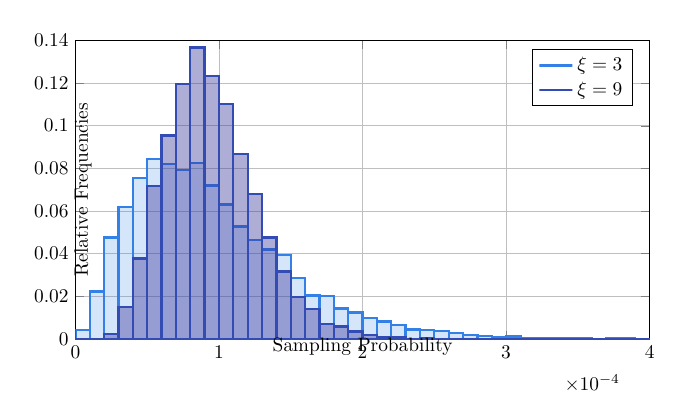
\begin{tikzpicture}[scale=0.7]
\begin{axis}[
    legend cell align={left},
    tick scale binop=\times,
    width=12cm, % Adjust the width
    height=7cm, % Adjust the height
    xlabel={Sampling Probability},
    ylabel={Relative Frequencies},
                  y label style={at={(axis description cs:0.04,.5)}, anchor=south},
      x label style={at={(axis description cs:0.5,0.025)}, anchor=north},
    %title={Comparison of Probability Distributions},
    grid=major,
    xmajorgrids=true,
    xminorgrids=false,
    ymajorgrids=true,
    yminorgrids=true,
    xtick={0, 1e-4, 2e-4, 3e-4, 4e-4},
    ytick={0, 0.02, 0.04, 0.06, 0.08, 0.1, 0.12, 0.14}, % Set y-axis ticks
    y tick label style={/pgf/number format/fixed}, % Force fixed-point notation
    yticklabels={0, 0.02, 0.04, 0.06, 0.08, 0.1, 0.12, 0.14}, 
    legend style={at={(0.97,0.97)},anchor=north east},
    legend cell align={left},
    xmin=0, xmax=4e-4,
    ymin=0, ymax=0.14,
    %ticklabel style={/pgf/number format/sci}
]

% Dirichlet(3) histogram
\addplot+[
    ybar interval,
    mark=no,
    fill={rgb,255:red,51;green,128;blue,230}, % Light blue
    fill opacity=0.2,
    draw={rgb,255:red,51;green,128;blue,230}, % Light blue
    line width=1.2pt
] coordinates {
(0.00000, 0.00437)
(1.00e-05, 0.02233)
(2.00e-05, 0.04760)
(3.00e-05, 0.06175)
(4.00e-05, 0.07543)
(5.00e-05, 0.08446)
(6.00e-05, 0.08189)
(7.00e-05, 0.07923)
(8.00e-05, 0.08265)
(9.00e-05, 0.07192)
(1.00e-04, 0.06308)
(1.10e-04, 0.05273)
(1.20e-04, 0.04646)
(1.30e-04, 0.04199)
(1.40e-04, 0.03952)
(1.50e-04, 0.02860)
(1.60e-04, 0.02033)
(1.70e-04, 0.02014)
(1.80e-04, 0.01435)
(1.90e-04, 0.01245)
(2.00e-04, 0.00979)
(2.10e-04, 0.00817)
(2.20e-04, 0.00646)
(2.30e-04, 0.00447)
(2.40e-04, 0.00418)
(2.50e-04, 0.00390)
(2.60e-04, 0.00285)
(2.70e-04, 0.00200)
(2.80e-04, 0.00143)
(2.90e-04, 0.00095)
(3.00e-04, 0.00114)
(3.10e-04, 0.00057)
(3.20e-04, 0.00038)
(3.30e-04, 0.00048)
(3.40e-04, 0.00048)
(3.50e-04, 0.00029)
(3.60e-04, 0.00000)
(3.70e-04, 0.00048)
(3.80e-04, 0.00019)
(3.90e-04, 0.00010)
(4.0e-04, 0.00000)
};

% Dirichlet(9) histogram
\addplot+[
    ybar interval,
    mark=no,
    fill={rgb,255:red,51;green,51;blue,153}, % Dark blue
    fill opacity=0.4,
    draw={rgb,255:red,51;green,76;blue,179}, % Slightly lighter dark blue
    line width=1.2pt
] coordinates {
    (0.00000, 0.00000)
(1.00e-05, 0.00000)
(2.00e-05, 0.00238)
(3.00e-05, 0.01511)
(4.00e-05, 0.03772)
(5.00e-05, 0.07163)
(6.00e-05, 0.09548)
(7.00e-05, 0.11961)
(8.00e-05, 0.13661)
(9.00e-05, 0.12322)
(1.00e-04, 0.11011)
(1.10e-04, 0.08683)
(1.20e-04, 0.06793)
(1.30e-04, 0.04760)
(1.40e-04, 0.03164)
(1.50e-04, 0.01967)
(1.60e-04, 0.01397)
(1.70e-04, 0.00694)
(1.80e-04, 0.00580)
(1.90e-04, 0.00352)
(2.00e-04, 0.00190)
(2.10e-04, 0.00105)
(2.20e-04, 0.00095)
(2.30e-04, 0.00000)
(2.40e-04, 0.00019)
(2.50e-04, 0.00000)
(2.60e-04, 0.00010)
(2.70e-04, 0.00000)
(2.80e-04, 0.00010)
(2.90e-04, 0.00000)
(3.00e-04, 0.00000)
(3.10e-04, 0.00000)
(3.20e-04, 0.00000)
(3.30e-04, 0.00000)
(3.40e-04, 0.00000)
(3.50e-04, 0.00000)
(3.60e-04, 0.00000)
(3.70e-04, 0.00000)
(3.80e-04, 0.00000)
(3.90e-04, 0.00000)
(4.0e-04, 0.00000)
};

\legend{$\xi=3$, $\xi=9$}

\end{axis}
\end{tikzpicture}
\caption{Normalized histograms of two probability vectors sampled from a symmetric $N$-dimensional Dirichlet distribution $\text{Dir}_N(\xi)$, with $N=10526$ and $\xi=3,9$.}
\label{fig1}
%\vspace{-0.6cm}
\end{figure}

%\vspace{-0.3cm}
\begin{figure}[h!]
\centering
%\minipage{0.5\columnwidth}
\begin{subfigure}[b]{\columnwidth}
\centering
  %%%%% First TikZ picture starts %%%%%
  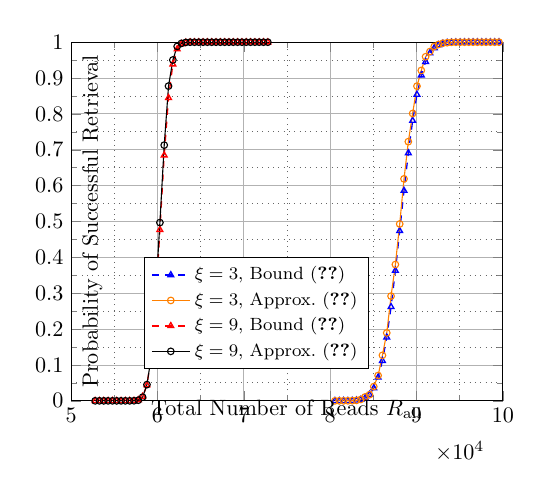
\begin{tikzpicture}[scale=0.8]
  \begin{axis}[
    legend cell align={left},
    %width=11cm, % Adjust the width
    %height=8cm, % Adjust the height
    tick scale binop=\times,
              y label style={at={(axis description cs:0.09,.5)}, anchor=south},
      x label style={at={(axis description cs:0.5,0.025)}, anchor=north},
    xlabel={Total Number of Reads $R_{\text{all}}$ },
    ylabel={Probability of Successful Retrieval},
    xticklabel={\pgfmathparse{\tick/1e-1}\pgfmathprintnumber{\pgfmathresult}},
    xtick scale label code/.code={$\times 10^4$}, % Custom multiplier
    %every x tick scale label/.style={at={(xticklabel cs:1)},anchor=south west},
    grid=both,
    ytick = {0, 0.1, 0.2, 0.3, 0.4, 0.5, 0.6, 0.7, 0.8, 0.9, 1},
    %xtick={0.001, 0.002, 0.003, 0.004, 0.005, 0.006, 0.007, 0.008, 0.009,
    %0.01},
    %ytick={20,40,60,80,100,120,140},
    % legend style={
    % at={(0.27,0.5)}, % Place the legend to the right of the plot
    % anchor=west,     % Align the left edge of the legend to the right of the plot   % Adjust legend font size
    % },
    legend style={at={(0.69,0.4)}, font=\footnotesize},
    legend style={font=\footnotesize},
    ymin = 0,
    ymax = 1,
    xmax = 100000,
    xmin = 50000,
    minor x tick num=1,
    minor y tick num=1,
    %cycle list name=color list,
    xmajorgrids=true,
    xminorgrids=true,
    ymajorgrids=true,
    yminorgrids=true,
    major grid style={black!30}, % Adjust major grid style
    minor grid style={dotted,black!60}, % Adjust minor grid style
]

\addplot+[color=blue, dashed, mark=triangle,mark size=1.5, mark options={solid, fill=none},line width=0.6pt, ] coordinates {
(80550, 2.41e-06)
(81050, 1.04e-05)
(81550, 4.06e-05)
(82050, 0.000142422)
(82550, 0.000451456)
(83050, 0.001297704)
(83550, 0.003392765)
(84050, 0.00809238)
(84550, 0.017665015)
(85050, 0.035407634)
(85550, 0.06539322)
(86050, 0.111693761)
(86550, 0.177140445)
(87050, 0.26198938)
(87550, 0.363070913)
(88050, 0.473925673)
(88550, 0.58604123)
(89050, 0.69079274)
(89550, 0.781360569)
(90050, 0.85394211)
(90550, 0.907945341)
(91050, 0.945308298)
(91550, 0.969383038)
(92050, 0.983851971)
(92550, 0.991974789)
(93050, 0.99624057)
(93550, 0.998339144)
(94050, 0.999307605)
(94550, 0.999727419)
(95050, 0.999898587)
(95550, 0.999964313)
(96050, 0.999988111)
(96550, 0.999996246)
(97050, 0.999998875)
(97550, 0.999999679)
(98050, 0.999999912)
(98550, 0.999999976)
(99050, 0.999999993)
(99550, 0.999999997)
(100050, 0.999999998)
(100550, 0.999999998)
};

\addplot+[color=orange,mark=o,mark size=1.5, mark options={fill=none},line width=0.5pt] coordinates {
(80550, 1.8e-06)
(81050, 8.62e-06)
(81550, 4.04e-05)
(82050, 0.000124)
(82550, 0.00044)
(83050, 0.0013)
(83550, 0.004)
(84050, 0.011)
(84550, 0.0171)
(85050, 0.039685381)
(85550, 0.07060525)
(86050, 0.126927413)
(86550, 0.189447319)
(87050, 0.292049752)
(87550, 0.380081425)
(88050, 0.4931471)
(88550, 0.618936146)
(89050, 0.722646758)
(89550, 0.801257857)
(90050, 0.877376182)
(90550, 0.92119907)
(91050, 0.959467628)
(91550, 0.973804834)
(92050, 0.988066533)
(92550, 0.993647975)
(93050, 0.997170556)
(93550, 0.998554112)
(94050, 0.999627335)
(94550, 0.999864077)
(95050, 0.999904932)
(95550, 0.999979046)
(96050, 0.999996094)
(96550, 0.999998716)
(97050, 0.999999751)
(97550, 0.999999934)
(98050, 0.99999999)
(98550, 0.999999996)
(99050, 1)
(99550, 1)
(100050, 1)
(100550, 1)
};

\addplot+[color=red, dashed, mark=triangle,mark size=1.5, mark options={solid, fill=none},line width=0.6pt] coordinates {
(52777, 3.62e-19)
(53277, 9.65e-17)
(53777, 1.54e-14)
(54277, 1.53e-12)
(54777, 9.85e-11)
(55277, 4.21e-09)
(55777, 1.22e-07)
(56277, 2.42e-06)
(56777, 3.35e-05)
(57277, 0.000327624)
(57777, 0.002292183)
(58277, 0.011664794)
(58777, 0.043918722)
(59277, 0.124751497)
(59777, 0.273644205)
(60277, 0.477015421)
(60777, 0.684767737)
(61277, 0.844806229)
(61777, 0.938516879)
(62277, 0.980550286)
(62777, 0.99510142)
(63277, 0.999017564)
(63777, 0.999842761)
(64277, 0.999979846)
(64777, 0.999997921)
(65277, 0.999999825)
(65777, 0.999999987)
(66277, 0.999999998)
(66777, 0.999999998)
(67277, 0.999999998)
(67777, 0.999999998)
(68277, 0.999999998)
(68777, 0.999999999)
(69277, 0.999999999)
(69777, 0.999999999)
(70277, 0.999999999)
(70777, 0.999999999)
(71277, 0.999999999)
(71777, 0.999999999)
(72277, 0.999999999)
(72777, 0.999999999)
};

\addplot+[color=black,mark=o,mark size=1.5, mark options={fill=none},line width=0.5pt] coordinates {
(52777, 8.96e-23)
(53277, 1.13e-19)
(53777, 7.32e-17)
(54277, 6.83e-14)
(54777, 1.57e-11)
(55277, 2.24e-09)
(55777, 5.38e-08)
(56277, 1.11e-06)
(56777, 1.95e-05)
(57277, 0.000288636)
(57777, 0.001851949)
(58277, 0.010223039)
(58777, 0.045203626)
(59277, 0.123201515)
(59777, 0.292397748)
(60277, 0.49700592)
(60777, 0.712936265)
(61277, 0.877615708)
(61777, 0.950359924)
(62277, 0.988133793)
(62777, 0.996707435)
(63277, 0.99939433)
(63777, 0.999956954)
(64277, 0.999990518)
(64777, 0.999999347)
(65277, 0.999999961)
(65777, 0.999999999)
(66277, 1)
(66777, 1)
(67277, 1)
(67777, 1)
(68277, 1)
(68777, 1)
(69277, 1)
(69777, 1)
(70277, 1)
(70777, 1)
(71277, 1)
(71777, 1)
(72277, 1)
(72777, 1)
};

\legend{}
\addlegendentry{$\xi=3$, Bound~\eqref{eqLBr}}
\addlegendentry{$\xi=3$, Approx.~\eqref{eqpR}}
\addlegendentry{$\xi=9$, Bound~\eqref{eqLBr}}
\addlegendentry{$\xi=9$, Approx.~\eqref{eqpR}}

\end{axis}
  \end{tikzpicture}
  %%%%% First Tiki picture ends %%%%%
  \caption{}
  \label{fig2a}
 % \endminipage 
  \vspace{0.3cm}
 \end{subfigure}
 %\hfill

  %\hspace{0.05\columnwidth}
%\minipage{0.5\columnwidth}
\begin{subfigure}[b]{\columnwidth}
\centering
  %%%%% Second TikZ picture starts %%%%%
  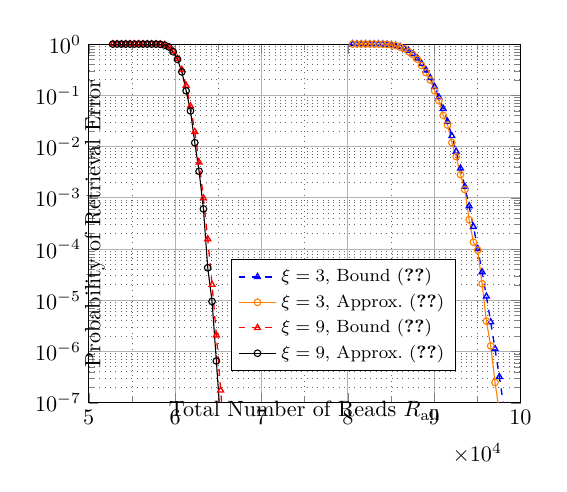
\begin{tikzpicture}[scale=0.8]
  \begin{semilogyaxis}[
    legend cell align={left},
    %width=11cm, % Adjust the width
    %height=8cm, % Adjust the height
    tick scale binop=\times,
              y label style={at={(axis description cs:0.055,.5)}, anchor=south},
      x label style={at={(axis description cs:0.5,0.025)}, anchor=north},
    xlabel={Total Number of Reads $R_{\text{all}}$ },
    ylabel={Probability of Retrieval Error},
    xticklabel={\pgfmathparse{\tick/1e-1}\pgfmathprintnumber{\pgfmathresult}},
    xtick scale label code/.code={$\times 10^4$}, % Custom multiplier
    %every x tick scale label/.style={at={(xticklabel cs:1)},anchor=south west},
    grid=both,
    %xtick={0.001, 0.002, 0.003, 0.004, 0.005, 0.006, 0.007, 0.008, 0.009,
    %0.01},
    %ytick={20,40,60,80,100,120,140},
    % legend style={
    % at={(0.27,0.5)}, % Place the legend to the right of the plot
    % anchor=west,     % Align the left edge of the legend to the right of the plot   % Adjust legend font size
    % },
    ymin=1e-7,
    ymax=1,
    xmax=100000,
    xmin=50000,
    minor x tick num=1,
    legend style={at={(0.85,0.4)}, font=\footnotesize},
    %cycle list name=color list,
    xmajorgrids=true,
    xminorgrids=true,
    ymajorgrids=true,
    yminorgrids=true,
    major grid style={black!30}, % Adjust major grid style
    minor grid style={dotted,black!60}, % Adjust minor grid style
]

\addplot+[color=blue, dashed, mark=triangle,mark size=1.5, mark options={solid, fill=none},line width=0.6pt, ] coordinates {
(80550, 0.99999759)
(81050, 0.9999896)
(81550, 0.9999594)
(82050, 0.999857578)
(82550, 0.999548544)
(83050, 0.998702296)
(83550, 0.996607235)
(84050, 0.99190762)
(84550, 0.982334985)
(85050, 0.964592366)
(85550, 0.93460678)
(86050, 0.888306239)
(86550, 0.822859555)
(87050, 0.73801062)
(87550, 0.636929087)
(88050, 0.526074327)
(88550, 0.41395877)
(89050, 0.30920726)
(89550, 0.218639431)
(90050, 0.14605789)
(90550, 0.092054659)
(91050, 0.054691702)
(91550, 0.030616962)
(92050, 0.016148029)
(92550, 0.008025211)
(93050, 0.00375943)
(93550, 0.001660856)
(94050, 0.000692395)
(94550, 0.000272581)
(95050, 0.000101413)
(95550, 3.5687e-05)
(96050, 1.1889e-05)
(96550, 3.754e-06)
(97050, 1.125e-06)
(97550, 3.21e-07)
(98050, 8.799999995e-08)
(98550, 2.399999999e-08)
(99050, 7.000000024e-09)
(99550, 3.000000026e-09)
(100050, 2.000000054e-09)
(100550, 2.000000054e-09)
};

\addplot+[color=orange,mark=o,mark size=1.5, mark options={fill=none},line width=0.5pt] coordinates {
(80550, 0.9999982)
(81050, 0.99999138)
(81550, 0.9999596)
(82050, 0.999876)
(82550, 0.99956)
(83050, 0.9987)
(83550, 0.996)
(84050, 0.989)
(84550, 0.9829)
(85050, 0.960314619)
(85550, 0.92939475)
(86050, 0.873072587)
(86550, 0.810552681)
(87050, 0.707950248)
(87550, 0.619918575)
(88050, 0.5068529)
(88550, 0.381063854)
(89050, 0.277353242)
(89550, 0.198742143)
(90050, 0.122623818)
(90550, 0.07880093)
(91050, 0.040532372)
(91550, 0.026195166)
(92050, 0.011933467)
(92550, 0.006352025)
(93050, 0.002829444)
(93550, 0.001445888)
(94050, 0.000372665)
(94550, 0.000135923)
(95050, 9.5068e-05)
(95550, 2.0954e-05)
(96050, 3.906e-06)
(96550, 1.284e-06)
(97050, 2.49e-07)
(97550, 6.600000002e-08)
(98050, 1.000000005e-08)
(98550, 3.999999998e-09)
(99050, 0)
(99550, 0)
(100050, 0)
(100550, 0)
};

\addplot+[color=red, dashed, mark=triangle,mark size=1.5, mark options={solid, fill=none},line width=0.6pt] coordinates {
(52777, 1)
(53277, 1)
(53777, 1)
(54277, 1)
(54777, 0.9999999999)
(55277, 0.9999999958)
(55777, 0.999999878)
(56277, 0.99999758)
(56777, 0.9999665)
(57277, 0.999672376)
(57777, 0.997707817)
(58277, 0.988335206)
(58777, 0.956081278)
(59277, 0.875248503)
(59777, 0.726355795)
(60277, 0.522984579)
(60777, 0.315232263)
(61277, 0.155193771)
(61777, 0.061483121)
(62277, 0.019449714)
(62777, 0.00489858)
(63277, 0.000982436)
(63777, 0.000157239)
(64277, 2.0154e-05)
(64777, 2.079e-06)
(65277, 1.75e-07)
(65777, 1.299999997e-08)
(66277, 2.000000054e-09)
(66777, 2.000000054e-09)
(67277, 2.000000054e-09)
(67777, 2.000000054e-09)
(68277, 2.000000054e-09)
(68777, 9.999999717e-10)
(69277, 9.999999717e-10)
(69777, 9.999999717e-10)
(70277, 9.999999717e-10)
(70777, 9.999999717e-10)
(71277, 9.999999717e-10)
(71777, 9.999999717e-10)
(72277, 9.999999717e-10)
(72777, 9.999999717e-10)
};

\addplot+[color=black,mark=o,mark size=1.5, mark options={fill=none},line width=0.5pt] coordinates {
(52777, 1)
(53277, 1)
(53777, 1)
(54277, 1)
(54777, 1)
(55277, 0.9999999978)
(55777, 0.9999999462)
(56277, 0.99999889)
(56777, 0.9999805)
(57277, 0.999711364)
(57777, 0.998148051)
(58277, 0.989776961)
(58777, 0.954796374)
(59277, 0.876798485)
(59777, 0.707602252)
(60277, 0.50299408)
(60777, 0.287063735)
(61277, 0.122384292)
(61777, 0.049640076)
(62277, 0.011866207)
(62777, 0.003292565)
(63277, 0.00060567)
(63777, 4.3046e-05)
(64277, 9.482e-06)
(64777, 6.53e-07)
(65277, 3.900000001e-08)
(65777, 9.999999717e-10)
(66277, 0)
(66777, 0)
(67277, 0)
(67777, 0)
(68277, 0)
(68777, 0)
(69277, 0)
(69777, 0)
(70277, 0)
(70777, 0)
(71277, 0)
(71777, 0)
(72277, 0)
(72777, 0)
};

\legend{}
\addlegendentry{$\xi=3$, Bound~\eqref{eqLBr}}
\addlegendentry{$\xi=3$, Approx.~\eqref{eqpR}}
\addlegendentry{$\xi=9$, Bound~\eqref{eqLBr}}
\addlegendentry{$\xi=9$, Approx.~\eqref{eqpR}}


\end{semilogyaxis}
  \end{tikzpicture}
  %%%%% Second TikZ picture ends %%%%%
  \caption{}
  \label{fig2b}
  \end{subfigure}
    %\endminipage
\caption{Probabilities of (a) successful retrieval and (b) retrieval error versus total number of reads $R_{\text{all}}$ for the two sampling probability vectors whose histograms are shown in Fig.~\ref{fig1}.}
\label{fig2}
%\vspace{-0.3cm}
\end{figure}


We analyze the probability of successful retrieval as a function total number of reads $R_{\text{all}}$, using: \begin{enumerate*}[label={\textit{(\roman*)}}] \item the analytical lower bound in~\eqref{eqLBr} evaluated for $\lambda=R_{\text{all}}$, $r'=2$, and subsets that truncate the summations where the tail probabilities are negligible; and \item a numerical approximation of~\eqref{eqpR} obtained by computing the empirical mean of $P_{\text{succ} \mid \boldsymbol{r}}$ over $10^{3}$ read profiles \( \boldsymbol{r} \) drawn from the multinomial distribution. \end{enumerate*} We consider two values of $\xi$, $\xi=3$ and $\xi=9$, to explore how different levels of bias impact data retrieval. The results in Fig.~\ref{fig2} show that probability of successful retrieval exhibits a sigmoidal behavior with respect to $R_{\text{all}}$, rising quickly to one near a threshold (Fig.~\ref{fig2a}), and causing the retrieval error probability to drop sharply (Fig.~\ref{fig2b}). The results also show good agreement between the analytical lower bound and the numerical approximation, highlighting the effectiveness of the bound. Furthermore, when $\xi=3$, a significantly higher number of reads is required for reliable retrieval compared to $\xi=9$, due to the stronger skew in sampling probabilities (Fig.~\ref{fig1}).

%\begin{multline} \label{eqRecc}
%g_j(h_0,\tilde{h}_{r'})= (1-q^{(j)}_{0}-q^{(j)}_{r'} )g_{j-1}(h_0,\tilde{h}_{r'}) \\ +q^{(j)}_{r'} g_{j-1}(h_0,\tilde{h}_{r'}-1) + q^{(j)}_{0} g_{j-1}(h_0-1,\tilde{h}_{r'}-1),
%\end{multline}
%\begin{multline} \label{eqRecc}
%\Pr(\rv{H}_{0,j}=h_{0}, \tilde{\rv{H}}_{r',j} = \tilde{h}_{r'})= q^{(j)}_{r'} \Pr(\rv{H}_{0,j-1}=h_{0}, \tilde{\rv{H}}_{r',j-1} = \tilde{h}_{r'}-1) \\ + q^{(j)}_{0} \Pr(\rv{H}_{0,j-1}=h_{0}-1, \tilde{\rv{H}}_{r',j-1} = \tilde{h}_{r'}-1) \\ 
%+(1-q^{(j)}_{0}-q^{(j)}_{r'} ) \Pr(\rv{H}_{0,j-1}=h_{0}, \tilde{\rv{H}}_{r',j-1} = \tilde{h}_{r'}),
%\end{multline}

%\begin{figure*}
%\begin{equation}
%\Pr(\rv{H}_{0,l+1}=h_{0}, \tilde{\rv{H}}_{r',l+1} = \tilde{h}_{r'})= q^{(l+1)}_{r'} \Pr(\rv{H}_{0,l}=h_{0}, \tilde{\rv{H}}_{r',l} = \tilde{h}_{r'}-1) + q^{(l+1)}_{0} \Pr(\rv{H}_{0,l}=h_{0}-1, \tilde{\rv{H}}_{r',l} = \tilde{h}_{r'}-1) +(1-q^{(l+1)}_{0}-q^{(l+1)}_{r'} ) \Pr(\rv{H}_{0,l}=h_{0}, \tilde{\rv{H}}_{r',l} = \tilde{h}_{r'}).
%\end{equation}
%\end{figure*}

%This model simplifies the analysis through Poissonization, which results in the number of reads per strand becoming {\em independent} Poisson random variables. As previously noted, Poissonization is not just a theoretical convenience but also a reliable approximation to the multinomial model when $R_{\text{\normalfont all}}$ is large and the sampling probabilities are small—a regime typical for large DNA pools.

%To account for such biases, we model $\boldsymbol{p}$ as being drawn from a symmetric Dirichlet distribution with concentration parameter $\xi > 0$. The Dirichlet distribution serves as a prior for the multinomial distribution, with smaller values of $\xi$ (approaching zero) corresponding to highly skewed sampling probabilities, while $\xi = \infty$ corresponds to uniform sampling. Importantly, this Multinomial-Dirichlet framework produces a positively skewed coverage distribution characterized by a long tail of few strands with high coverage, consistent with typical empirical observations~\cite{gimpel2023digital}. By varying $\xi$, we can systematically analyze how different levels of coverage bias influence the data retrieval process.
%
%Evaluating the exact value of $P_{\text{succ}\mid\boldsymbol{p}}(R)$ from~\eqref{eqpR} is computationally infeasible, even for moderate values of $N$ and $R$. A practical alternative is to approximate it numerically using Monte Carlo methods, which involves computing the empirical mean of \( P_{\text{succ} \mid \boldsymbol{r}} \) over a large number of read profiles \( \boldsymbol{r} \) sampled from the multinomial distribution. Furthermore, an interesting application of this framework is determining the minimum number of reads $R$ required to ensure successful data retrieval with a probability exceeding a user-defined threshold. For such use cases, it suffices to have a good lower bound on $P_{\text{succ}\mid\boldsymbol{p}}(R)$, even if its exact value cannot be computed. To this end, we present an analytical lower bound on $ P_{\text{succ}\mid\boldsymbol{p}}(R) $, which can be efficiently computed.


%\begin{proof}
%Recall that
%\begin{equation}
%P_{\text{succ}\mid \boldsymbol{r}}=\Pr\left(\rv{S}_N{(\boldsymbol{r})}\geq K \right),
%\end{equation}
%where $\rv{S}_N{(\boldsymbol{r})} =\rv{Z}_1{(r_1)}+\rv{Z}_2{(r_2)}+\ldots+\rv{Z}_N{(r_N)}$. For a given read profile $\boldsymbol{r}=(r_1,\ldots,r_N)$, let $\Tilde{\boldsymbol{r}}=(\Tilde{r}_1,\Tilde{r}_2,\ldots,\Tilde{r}_N)$ represent the elements of $\boldsymbol{r}$ sorted in increasing order. Due to the symmetry with respect to the strands, it holds that
%\begin{equation}
%    \rv{S}_N{(\boldsymbol{r})} = \rv{S}_N{(\Tilde{\boldsymbol{r}})} =\rv{Z}_1{(\Tilde{r}_1)}+\rv{Z}_2{(\Tilde{r}_2)}+\ldots+\rv{Z}_N{(\Tilde{r}_N)}.
%\end{equation}
%% For a given read profile $\boldsymbol{r}=(r_1,\ldots,r_N)$ and $r' \in [R]$ , let $(j_1,j_2,\ldots,j_N)$ be a permutation of $[N]$ satisfying
%% $$r_{j_1} \leq r_{j_2} \leq \ldots \leq r_{j_{N'}} \leq r' < r_{j_{N'+1}}\leq \ldots \leq r_{j_N},$$
%% where $N'\leq N$ is the number of strands that are read less than or equal to $r'$ times.
%For any $r' \in [R]$, $N'=h_0+h_1+\ldots+h_{r'}$ denotes the number of strands that are read less than or equal to $r'$ times. For given values of $r'$, $N'$, $h_0$, and $\Tilde{\boldsymbol{r}}$, we define the following random variables
%\begin{align}
%\rv{S}_{\text{low}} &= \rv{Z}_1{(\Tilde{r}_1)}+\rv{Z}_2{(\Tilde{r}_2)}+\ldots+\rv{Z}_{N'}{(\Tilde{r}_{N'})}, \\
%   \rv{S}'_{\text{low}} &= \rv{Z}_{{h_0+1}}{(1)}+\rv{Z}_{{h_0+2}}{(1)}+\ldots+\rv{Z}_{N'}{(1)}, \\
%   \rv{S}_{\text{high}} &= \rv{Z}_{N'+1}{(\Tilde{r}_{N'+1})}+\ldots+\rv{Z}_N{(\Tilde{r}_N)}, \\
%   \rv{S}'_{\text{high}} &= \rv{Z}_{N'+1}{(r')}+\ldots+\rv{Z}_N{(r')}.
%\end{align}
%%$\rv{S}_N{(\boldsymbol{r})}=\rv{S}_{\text{low}}(\boldsymbol{r}_{[1,N']})+\rv{S}_{\text{high}}(\boldsymbol{r}_{[N'+1,N]})$. 
%We have
%\begin{align}
%    P_{\text{succ} \mid  \boldsymbol{r}} &= \Pr\left(\rv{S}_N{(\boldsymbol{r})}\geq K \right), \\
%    &= \Pr\left(\rv{S}_{\text{low}}+\rv{S}_{\text{high}}\geq K \right), \\
%    &\geq \Pr \left(\rv{S}'_{\text{low}} + \rv{S}'_{\text{high}} \geq K \right), \\
%    &= \sum_{s\in \mathcal{S}}  \Pr (\rv{S}'_{\text{high}} \geq K-s \mid \rv{S}'_{\text{low}}=s ) \Pr(\rv{S}'_{\text{low}} = s),~~~~~~~~~~~~
%\end{align}
%which concludes the proof.
%\end{proof}

\section{Optimization and Trade-offs} \label{opt}
In this section, we apply the theoretical framework developed in Section~\ref{sec3} to analyze the trade‐offs between various design factors that affect the reliability of data retrieval under MDS coding. Our goal is to identify optimal operating points that minimize sequencing or synthesis costs under reliability constraints. Specifically, we focus on two key optimization problems: \begin{enumerate*}[label={\textit{(\roman*)}}] \item minimizing the number of reads needed for retrieval (sequencing cost); and \item maximizing the information density achieved by the inner+outer code combination (synthesis cost);\end{enumerate*} both while ensuring a target success probability of at least $1-\delta_{\text{th}}$. We fix $\delta_{\text{th}}=10^{-6}$ throughout this section, and consider the same initial configuration as in Section~\ref{example}, with $K=10000$, $k=360$, $m=8$, $\epsilon=0.01$. To evaluate the optimal operating points, we use our analytical lower bound on the probability of success in~\eqref{eqLBr} (parametrized same as in Section~\ref{example}), and apply a grid search over the relevant parameters. %Below, we first focus on determining the minimum read depth required for reliable retrieval which is relevant to sequencing costs, and then investigate how best to allocate redundancy among the inner and outer MDS codes.

\subsection{Minimum Number of Reads for Reliable Retrieval} \label{sec4a}
We quantify the minimum achievable sequencing cost through $R^{\star}_{\text{all}}/K$, where $R^{\star}_{\text{all}}$ is the minimum number of reads needed to achieve successful retrieval with a probability exceeding the target threshold, and $K$ is the number of information strands. We refer to $R_{\text{all}}/K$ as the {\em information} read depth, which must be at least one to ensure a non-zero probability of successful retrieval. Note that this metric differs from the commonly used coverage depth, typically defined as $R_{\text{all}}/N$, where $N$ is the total number of stored strands, and for which information retrieval can theoretically be achieved even when this quantity is less than one.

Fig.~\ref{fig3a} illustrates the impact of the outer MDS code rate $\rho_{\text{out}}$ on~$R^{\star}_{\text{all}}/K$ for different inner MDS code rates $\rho_{\text{in}}$. For $\rho_{\text{in}}=0.96$ and $0.92$, the sequencing cost $R^{\star}_{\text{all}}/K$ decreases as more redundancy is introduced through the outer code, but with diminishing returns, which is consistent with findings in the literature~\cite{10750859,abraham2024covering,10619151}. Interestingly, for $\rho_{\text{in}}=1$, we observe that adding redundancy in the outer code can actually hurt beyond a certain point. The intuition here is that when $N$ is large (i.e., $\rho_{\text{out}}$ is small), the reads become so thinly spread out that the reliability of decoding individual strands drops significantly. Since the inner code provides no additional protection when $\rho_{\text{in}}=1$, the noisiness of individual strands dominates, thus requiring a higher number of reads to compensate for this degradation. Fig.~\ref{fig3b} examines the effect of the Dirichlet bias parameter $\xi$, which governs the skewness of the sampling probabilities. As expected, the results demonstrate that bias can noticeably increase sequencing costs for reliable~retrieval.

\begin{remark}
    Previous works have studied the problem of coding for minimizing the sequencing coverage depth \cite{10750859,abraham2024covering,10619151}, focusing on how introducing redundancy in the outer code can reduce the coverage depth required for data retrieval, and on designing codes that achieve this reduction. These studies assumed noiseless strands during retrieval, leading to the conclusion that increasing redundancy always lowers the required coverage depth (i.e., the minimum coverage is attained as $\rho_{\text{out}}\to 0$). However, our analysis reveals a more nuanced behavior in the presence of noise. Specifically, the results in Fig.~\ref{fig3a}  show that the optimal point does not always occur when the outer code operates at its lowest rate. This insight opens new directions for future work on coding for minimizing sequencing costs under noisy conditions.
\end{remark}

\begin{figure}[h!]
%\vspace{-0.4cm}
\centering
%\minipage{0.5\columnwidth}
\begin{subfigure}[b]{\columnwidth}
\centering
  %%%%% First TikZ picture starts %%%%%
  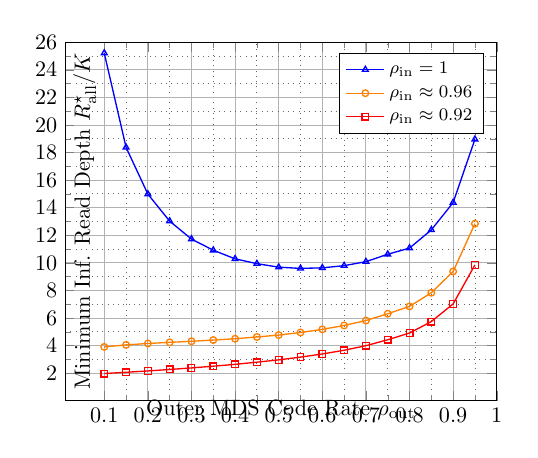
\begin{tikzpicture}[scale=0.8]
  \begin{axis}[
    legend cell align={left},
    %width=11cm, % Adjust the width
    %height=8cm, % Adjust the height
          y label style={at={(axis description cs:0.09,.5)}, anchor=south},
      x label style={at={(axis description cs:0.5,0.025)}, anchor=north},
    tick scale binop=\times,
          grid=major, 
      minor tick num=1,
    xlabel={Outer MDS Code Rate $\rho_{\text{out}}$},
    ylabel={Minimum Inf. Read Depth $R^{\star}_{\text{all}}/K$},
    %xticklabel={\pgfmathparse{\tick/1e-1}\pgfmathprintnumber{\pgfmathresult}},
    %xtick scale label code/.code={$\times 10^4$}, % Custom multiplier
    %every x tick scale label/.style={at={(xticklabel cs:1)},anchor=south west},
    grid=both,
    %xtick={0.001, 0.002, 0.003, 0.004, 0.005, 0.006, 0.007, 0.008, 0.009,
    %0.01},
    ytick={2,4,6,8,10,12,14,16,18,20,22,24,26},
    xtick={0.1,0.2,0.3,0.4,0.5,0.6,0.7,0.8,0.9,1},
    % legend style={
    % at={(0.27,0.5)}, % Place the legend to the right of the plot
    % anchor=west,     % Align the left edge of the legend to the right of the plot   % Adjust legend font size
    % },
    legend pos=north east,
    legend style={font=\footnotesize},
    ymin = 0,
    ymax = 26,
    xmax = 1,
    %ymax = 1,
    %cycle list name=color list,
    xmajorgrids=true,
    xminorgrids=true,
    ymajorgrids=true,
    yminorgrids=true,
    major grid style={black!30}, % Adjust major grid style
    minor grid style={dotted,black!60}, % Adjust minor grid style
]

\addplot+[color=blue, mark=triangle,mark size=1.5, mark options={solid, fill=none},line width=0.6pt, ] coordinates {
(0.1, 25.211)
(0.15, 18.3742)
(0.2, 14.9859)
(0.25, 13.0258)
(0.3, 11.7267)
(0.35, 10.9184)
(0.4, 10.2934)
(0.45, 9.9446)
(0.5, 9.6911)
(0.55, 9.6003)
(0.6, 9.642)
(0.65, 9.799)
(0.7, 10.0898)
(0.75, 10.6273)
(0.8, 11.0728)
(0.85, 12.3921)
(0.9, 14.3737)
(0.95, 18.9634)
};

\addplot+[color=orange,mark=o,mark size=1.5, mark options={fill=none},line width=0.6pt] coordinates {
(0.1, 3.9096)
(0.15, 4.0553)
(0.2, 4.1571)
(0.25, 4.2398)
(0.3, 4.3172)
(0.35, 4.4059)
(0.4, 4.502)
(0.45, 4.6292)
(0.5, 4.7685)
(0.55, 4.9558)
(0.6, 5.1819)
(0.65, 5.4636)
(0.7, 5.821)
(0.75, 6.3147)
(0.8, 6.8449)
(0.85, 7.8347)
(0.9, 9.3763)
(0.95, 12.8419)
};

\addplot+[color=red, mark=square,mark size=1.5, mark options={solid, fill=none},line width=0.6pt] coordinates {
(0.1, 1.9797)
(0.15, 2.0692)
(0.2, 2.1662)
(0.25, 2.2737)
(0.3, 2.3845)
(0.35, 2.5126)
(0.4, 2.6452)
(0.45, 2.8034)
(0.5, 2.9691)
(0.55, 3.1692)
(0.6, 3.397)
(0.65, 3.668)
(0.7, 3.9974)
(0.75, 4.4278)
(0.8, 4.9165)
(0.85, 5.7456)
(0.9, 7.0273)
(0.95, 9.8552)
};


\legend{}
 \addlegendentry{$\rho_{\text{\normalfont in}}=1$}
\addlegendentry{$\rho_{\text{\normalfont in}} \approx 0.96$}
 \addlegendentry{$\rho_{\text{\normalfont in}}\approx 0.92$}

\end{axis}
  \end{tikzpicture}
  %%%%% First Tiki picture ends %%%%%
  \caption{Dirichlet parameter $\xi=3.$}
  \label{fig3a}
 % \endminipage 
   \vspace{0.3cm}
 \end{subfigure}
 %\hfill
  %\hspace{0.05\columnwidth}
%\minipage{0.5\columnwidth}
\begin{subfigure}[b]{\columnwidth}
\centering
  %%%%% Second TikZ picture starts %%%%%
  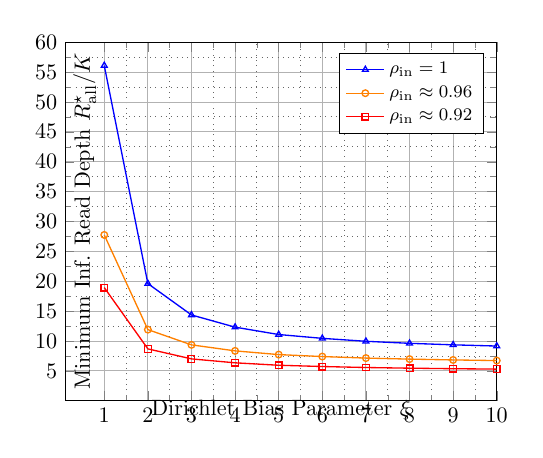
\begin{tikzpicture}[scale=0.8]
  \begin{axis}[
    legend cell align={left},
    %width=11cm, % Adjust the width
    %height=8cm, % Adjust the height
    tick scale binop=\times,
    xlabel={Dirichlet Bias Parameter $\xi$},
    ylabel={Minimum Inf. Read Depth $R^{\star}_{\text{all}}/K$},
          y label style={at={(axis description cs:0.09,.5)}, anchor=south},
      x label style={at={(axis description cs:0.5,0.025)}, anchor=north},
    %xticklabel={\pgfmathparse{\tick/1e-1}\pgfmathprintnumber{\pgfmathresult}},
    %xtick scale label code/.code={$\times 10^4$}, % Custom multiplier
    %every x tick scale label/.style={at={(xticklabel cs:1)},anchor=south west},
          grid=major, 
      minor tick num=1,
    grid=both,
    %xtick={0.001, 0.002, 0.003, 0.004, 0.005, 0.006, 0.007, 0.008, 0.009,
    %0.01},
    xtick={1,2,3,4,5,6,7,8,9,10},
    ytick={5,10,15,20,25,30,35,40,45,50,55,60},
    %xtick={0.1,0.2,0.3,0.4,0.5,0.6,0.7,0.8,0.9,1},
    % legend style={
    % at={(0.27,0.5)}, % Place the legend to the right of the plot
    % anchor=west,     % Align the left edge of the legend to the right of the plot   % Adjust legend font size
    % },
    legend pos=north east,
    legend style={font=\footnotesize},
    ymin = 0,
    %ymax = 26,
    xmax = 10,
    ymax=60,
    %ymax = 1,
    %cycle list name=color list,
    xmajorgrids=true,
    xminorgrids=true,
    ymajorgrids=true,
    yminorgrids=true,
    major grid style={black!30}, % Adjust major grid style
    minor grid style={dotted,black!60}, % Adjust minor grid style
]

\addplot+[color=blue, mark=triangle,mark size=1.5, mark options={solid, fill=none},line width=0.6pt, ] coordinates {
(1, 56.0934)
(2, 19.6147)
(3, 14.3657)
(4, 12.3249)
(5, 11.0913)
(6, 10.4514)
(7, 9.9607)
(8, 9.6204)
(9, 9.3666)
(10, 9.1652)
};

\addplot+[color=orange,mark=o,mark size=1.5, mark options={fill=none},line width=0.6pt] coordinates {
(1, 27.7549)
(2, 11.9123)
(3, 9.3621)
(4, 8.3578)
(5, 7.735)
(6, 7.4076)
(7, 7.1513)
(8, 6.9787)
(9, 6.8413)
(10, 6.7351)
};

\addplot+[color=red, mark=square,mark size=1.5, mark options={solid, fill=none},line width=0.6pt] coordinates {
(1, 18.9459)
(2, 8.6913)
(3, 7.016)
(4, 6.359)
(5, 5.9524)
(6, 5.7398)
(7, 5.5738)
(8, 5.462)
(9, 5.3742)
(10, 5.3058)
};


\legend{}
 \addlegendentry{$\rho_{\text{\normalfont in}}=1$}
\addlegendentry{$\rho_{\text{\normalfont in}} \approx 0.96$}
 \addlegendentry{$\rho_{\text{\normalfont in}}\approx 0.92$}

\end{axis}
  \end{tikzpicture}
  %%%%% Second TikZ picture ends %%%%%
  \caption{Outer code rate $\rho_{\text{out}}=0.9$.}
  \label{fig3b}
  \end{subfigure}
    %\endminipage
\caption{Minimum information read depth $R^{\star}_{\text{all}}/K$ versus (a) Outer MDS code rate $\rho_{\text{\normalfont out}}$; and (b) Dirichlet parameter $\xi$. The Dirichlet parameter is fixed to $\xi=3$ in (a), and the outer code rate is fixed to $\rho_{\text{\normalfont out}}=0.9$ in (b).}
\label{fig3}
%\vspace{-0.35cm}
\end{figure}



\subsection{Optimal Redundancy Allocation}\label{sec4b}
We measure the synthesis cost through the information density $\Delta= 2\rho_{\text{in}} \rho_{\text{out}} = 2(k/n)(K/N)$, and analyze the optimal redundancy allocation between the inner and outer code that maximizes $\Delta$ under the same reliability constraints considered previously. Fig.~\ref{fig4a} shows the optimal information density $\Delta^{\star}$ as a function of the information read depth $R_{\text{all}}/K$. Initially, a higher number of reads leads to a significant increase in $\Delta^{\star}$, but this trend eventually saturates due to diminishing returns. Our numerical results indicate that $\Delta^{\star}=1.99$ bits/NT is achievable for a read depth of~$\approx 60$. Fig.~\ref{fig4b} illustrates the interplay between the optimal code rates of the inner and outer MDS codes, $\rho^{\star}_{\text{in}}$ and $\rho^{\star}_{\text{out}}$, and plots the aggregate code rate $\rho^{\star}_{\text{in}} \rho^{\star}_{\text{out}}$. These results underscore the importance of inner codes in the low-read regime, as their contribution to enhancing reliability plays a pivotal role in minimizing synthesis costs.

\begin{figure}[h!]
%\vspace{-0.35cm}
\centering
%\minipage{0.5\columnwidth}
\begin{subfigure}[b]{\columnwidth}
\centering
  %%%%% First TikZ picture starts %%%%%
  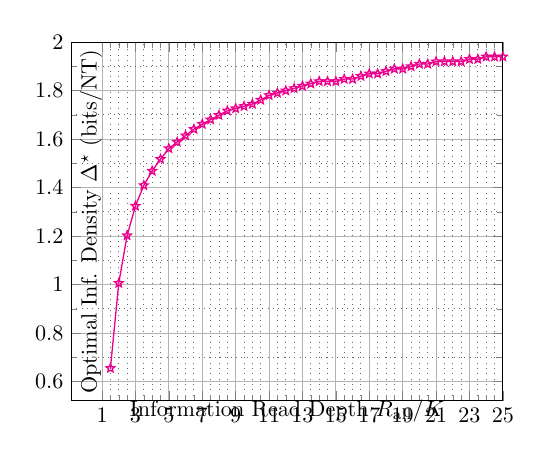
\begin{tikzpicture}[scale=0.8]
  \begin{axis}[
      legend cell align={left},
      tick scale binop=\times,
       %width=10cm, % Adjust the width
       %height=8cm, % Adjust the height
      xlabel={Information Read Depth $R_{\text{all}}/K$},
      ylabel={Optimal Inf. Density $\Delta^{\star}$ (bits/NT)},
      y label style={at={(axis description cs:0.09,.5)}, anchor=south},
      x label style={at={(axis description cs:0.5,0.025)}, anchor=north},
      grid=major, 
      minor y tick num=1,
      minor x tick num=3,
      grid=both,
      ytick = {0.6,0.8,1,1.2,1.4,1.6,1.8,2},
      xtick = {1,3,5,7,9,11,13,15,17,19,21,23,25},
      legend pos=north east,
      legend style={font=\footnotesize},
      xmax=25,
      ymax=2,
      xmajorgrids=true,
      xminorgrids=true,
      ymajorgrids=true,
      yminorgrids=true,
      major grid style={black!30},
      minor grid style={dotted,black!60},
    ]

\addplot+[color=magenta, mark=mystar,mark size=1.5, mark options={solid, fill=none},line width=0.6pt, ] coordinates {
(1.5, 0.655263158)
(2, 1.006363636)
(2.5, 1.202727273)
(3, 1.324528302)
(3.5, 1.409433962)
(4, 1.468867925)
(4.5, 1.517647059)
(5, 1.561764706)
(5.5, 1.588235294)
(6, 1.614705882)
(6.5, 1.641176471)
(7, 1.662244898)
(7.5, 1.680612245)
(8, 1.698979592)
(8.5, 1.717346939)
(9, 1.726530612)
(9.5, 1.735714286)
(10, 1.744897959)
(10.5, 1.761702128)
(11, 1.780851064)
(11.5, 1.790425532)
(12, 1.8)
(12.5, 1.809574468)
(13, 1.819148936)
(13.5, 1.828723404)
(14, 1.838297872)
(14.5, 1.838297872)
(15, 1.838297872)
(15.5, 1.84787234)
(16, 1.84787234)
(16.5, 1.86)
(17, 1.87)
(17.5, 1.87)
(18, 1.88)
(18.5, 1.89)
(19, 1.89)
(19.5, 1.9)
(20, 1.91)
(20.5, 1.91)
(21, 1.92)
(21.5, 1.92)
(22, 1.92)
(22.5, 1.92)
(23, 1.93)
(23.5, 1.93)
(24, 1.94)
(24.5, 1.94)
(25, 1.94)
};


  \end{axis}
  \end{tikzpicture}
  %%%%% First Tiki picture ends %%%%%
  \caption{}
  \label{fig4a}
 % \endminipage 
 \end{subfigure}
 %\hfill
 \vspace{0.3cm}
  %\hspace{0.05\columnwidth}
%\minipage{0.5\columnwidth}
\begin{subfigure}[b]{\columnwidth}
\centering
  %%%%% Second TikZ picture starts %%%%%
  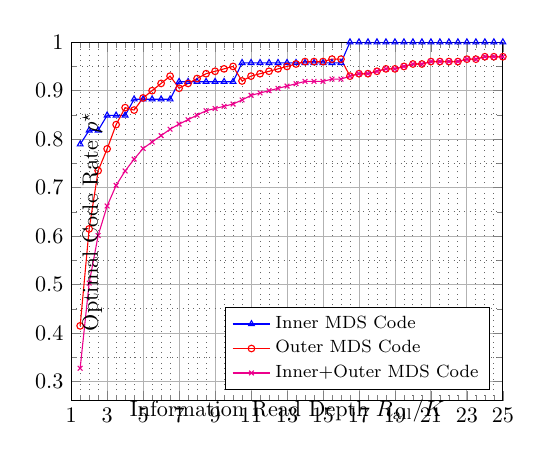
\begin{tikzpicture}[scale=0.8]
  \begin{axis}[
      legend cell align={left},
      tick scale binop=\times,
      xlabel={Information Read Depth $R_{\text{all}}/K$},
      ylabel={Optimal Code Rate $\rho^{\star}$},
       y label style={at={(axis description cs:0.09,.5)}, anchor=south},
             x label style={at={(axis description cs:0.5,0.025)}, anchor=north},
      grid=major, 
      minor y tick num=1,
      minor x tick num=3,
      grid=both,
      ytick = {0.3,0.4,0.5,0.6,0.7,0.8,0.9,1},
      xtick = {1,3,5,7,9,11,13,15,17,19,21,23,25},
      legend pos=south east,
      legend style={font=\footnotesize},
      xmax=25,
      xmin=1,
      ymax=1,
      xmajorgrids=true,
      xminorgrids=true,
      ymajorgrids=true,
      yminorgrids=true,
      major grid style={black!30},
      minor grid style={dotted,black!60},
    ]

    \addplot+[color=blue, mark=triangle,mark size=1.5, mark options={solid, fill=none},line width=0.5pt, ] coordinates {
(1.5, 0.789473684)
(2, 0.818181818)
(2.5, 0.818181818)
(3, 0.849056604)
(3.5, 0.849056604)
(4, 0.849056604)
(4.5, 0.882352941)
(5, 0.882352941)
(5.5, 0.882352941)
(6, 0.882352941)
(6.5, 0.882352941)
(7, 0.918367347)
(7.5, 0.918367347)
(8, 0.918367347)
(8.5, 0.918367347)
(9, 0.918367347)
(9.5, 0.918367347)
(10, 0.918367347)
(10.5, 0.957446809)
(11, 0.957446809)
(11.5, 0.957446809)
(12, 0.957446809)
(12.5, 0.957446809)
(13, 0.957446809)
(13.5, 0.957446809)
(14, 0.957446809)
(14.5, 0.957446809)
(15, 0.957446809)
(15.5, 0.957446809)
(16, 0.957446809)
(16.5, 1)
(17, 1)
(17.5, 1)
(18, 1)
(18.5, 1)
(19, 1)
(19.5, 1)
(20, 1)
(20.5, 1)
(21, 1)
(21.5, 1)
(22, 1)
(22.5, 1)
(23, 1)
(23.5, 1)
(24, 1)
(24.5, 1)
(25, 1)
};

\addplot+[color=red, mark=o,mark size=1.5, mark options={solid, fill=none},line width=0.5pt, ] coordinates {
(1.5, 0.415)
(2, 0.615)
(2.5, 0.735)
(3, 0.78)
(3.5, 0.83)
(4, 0.865)
(4.5, 0.86)
(5, 0.885)
(5.5, 0.9)
(6, 0.915)
(6.5, 0.93)
(7, 0.905)
(7.5, 0.915)
(8, 0.925)
(8.5, 0.935)
(9, 0.94)
(9.5, 0.945)
(10, 0.95)
(10.5, 0.92)
(11, 0.93)
(11.5, 0.935)
(12, 0.94)
(12.5, 0.945)
(13, 0.95)
(13.5, 0.955)
(14, 0.96)
(14.5, 0.96)
(15, 0.96)
(15.5, 0.965)
(16, 0.965)
(16.5, 0.93)
(17, 0.935)
(17.5, 0.935)
(18, 0.94)
(18.5, 0.945)
(19, 0.945)
(19.5, 0.95)
(20, 0.955)
(20.5, 0.955)
(21, 0.96)
(21.5, 0.96)
(22, 0.96)
(22.5, 0.96)
(23, 0.965)
(23.5, 0.965)
(24, 0.97)
(24.5, 0.97)
(25, 0.97)
};

\addplot+[color=magenta, mark=x,mark size=1.5, mark options={solid, fill=none},line width=0.5pt, ] coordinates {
(1.5, 0.327631579)
(2, 0.503181818)
(2.5, 0.601363636)
(3, 0.662264151)
(3.5, 0.704716981)
(4, 0.734433962)
(4.5, 0.758823529)
(5, 0.780882353)
(5.5, 0.794117647)
(6, 0.807352941)
(6.5, 0.820588235)
(7, 0.831122449)
(7.5, 0.840306122)
(8, 0.849489796)
(8.5, 0.858673469)
(9, 0.863265306)
(9.5, 0.867857143)
(10, 0.87244898)
(10.5, 0.880851064)
(11, 0.890425532)
(11.5, 0.895212766)
(12, 0.9)
(12.5, 0.904787234)
(13, 0.909574468)
(13.5, 0.914361702)
(14, 0.919148936)
(14.5, 0.919148936)
(15, 0.919148936)
(15.5, 0.92393617)
(16, 0.92393617)
(16.5, 0.93)
(17, 0.935)
(17.5, 0.935)
(18, 0.94)
(18.5, 0.945)
(19, 0.945)
(19.5, 0.95)
(20, 0.955)
(20.5, 0.955)
(21, 0.96)
(21.5, 0.96)
(22, 0.96)
(22.5, 0.96)
(23, 0.965)
(23.5, 0.965)
(24, 0.97)
(24.5, 0.97)
(25, 0.97)
};    
    % ... other \addplot commands ...

  \legend{}
  \addlegendentry{Inner MDS Code}
  \addlegendentry{Outer MDS Code}
  \addlegendentry{Inner+Outer MDS Code}
  \end{axis}
  \end{tikzpicture}
  %%%%% Second TikZ picture ends %%%%%
  \caption{}
  \label{fig4b}
  \end{subfigure}
    %\endminipage
\caption{Plot (a) shows the optimal information density \mbox{$\Delta^{\star}=2\rho_{\text{in}}^{\star}\rho_{\text{out}}^{\star}$} in bits/NT as a function of the information read depth; and (b) shows the corresponding optimal code rates $\rho_{\text{in}}^{\star}$, $\rho_{\text{out}}^{\star}$, and $\rho^{\star}=\rho_{\text{in}}^{\star}\rho_{\text{out}}^{\star}$. The Dirichlet parameter is fixed to  $\xi=3$.}
\label{fig4}
%\vspace{-0.2cm}
\end{figure}

In summary, our results highlight key trade-offs between design parameters that can be optimized to reduce sequencing or synthesis costs. To gain further insights into optimal DNA storage system design, it would be interesting to explore additional cost functions in future work, including ones that account for both synthesis and sequencing costs simultaneously.

\bibliographystyle{IEEEtran}
\bibliography{Refs}


%\newpage
%\onecolumn
\appendices
\section{Proof of Lemma~\ref{lemm1}}
Let $\tilde{\Rv{Y}}^{1}, \tilde{\Rv{Y}}^{2}, \ldots, \tilde{\Rv{Y}}^{r}\in \Sigma^{n/2}$ be the $r\in \mathbb{N}$ noisy copies generated by the channel corresponding to a given DNA strand $\tilde{\boldsymbol{x}} \in \Sigma^{n/2}$, where $\Sigma = \{\mathsf{A,C,G,T}\}$. For each position $i \in [n/2]$, the consensus nucleotide $\tilde{\rv{C}}_i\in \Sigma$ is chosen as the most frequent one among $\tilde{\rv{Y}}_i^{1},\tilde{\rv{Y}}_i^{2}, \ldots, \tilde{\rv{Y}}_i^{r}$, with ties broken uniformly at random. Since the QSC introduces i.i.d. errors and the consensus mechanism processes each nucleotide position independently, the errors in the consesnsus sequence also remain i.i.d., with error probability 
$$\epsilon_{(r)}=\Pr(\tilde{\rv{C}}_i \neq \tilde{x}_i), \quad \text{for any } i \in [n/2].$$
Due to the symmetry across positions, we drop the subscript $i$ in the rest of the proof. Let $(\rv{K}_1,\rv{K}_2,\rv{K}_3,\rv{K}_4)$ be the random vector defined as $$(\rv{K}_1,\rv{K}_2,\rv{K}_3,\rv{K}_4)\in \left\{ \boldsymbol{\kappa} \in \mathbb{N}^4 \ : \ \kappa_1 + \kappa_2 + \kappa_3 + \kappa_4 = r \right\},$$  where $$\rv{K}_1=\sum_{\ell=1}^r \mathds{1}_{\{\tilde{\rv{Y}}^{\ell} = \tilde{x}\}}$$ 
counts the number of copies in which the nucleotide $\tilde{x}$ is retained with no error, and $\rv{K}_2$,$\rv{K}_3$, and $\rv{K}_4$ count the number of copies in which $\tilde{x}$ is substituted to each of the other three nucleotides in $\Sigma \setminus \tilde{x}$. The vector $(\rv{K}_1,\rv{K}_2,\rv{K}_3,\rv{K}_4)$ follows a multinomial distribution with parameter $r$ (number of trials) and probability vector $(1-\epsilon,\frac{\epsilon}{3},\frac{\epsilon}{3},\frac{\epsilon}{3})$, where $\epsilon$ is the QSC error rate. For a realization $\boldsymbol{\kappa} = (\kappa_1, \kappa_2, \kappa_3, \kappa_4)$, the probability of correctly recovering $\tilde{x}$ via majority voting (with ties broken uniformly) is
$$\Pr(\tilde{\rv{C}} = \tilde{x} \mid \kappa_1,\kappa_2,\kappa_3,\kappa_4) = \frac{\mathds{1}_{\{\kappa_1 \geq \kappa_2,\kappa_3,\kappa_4\}}}{\sum_{i=1}^4 \mathds{1}_{\{\kappa_i = \kappa_1\}}}  ,
$$
where the denominator \mbox{$\omega_{(\boldsymbol{\kappa})} = \sum_{i=1}^4 \mathds{1}_{\{\kappa_i = \kappa_1\}}$} counts the number of ties. Applying the law of total probability,
\begin{align*}
  \Pr(\tilde{\rv{C}} = \tilde{x}) &=  \hspace{-0.75cm} \sum_{\substack{\boldsymbol{\kappa}\in \mathbb{N}^4 \\ \kappa_1+\kappa_2+\kappa_3+\kappa_4=r}} \hspace{-0.75cm}  \Pr(\tilde{\rv{C}} = \tilde{x} \mid \kappa_1,\kappa_2,\kappa_3,\kappa_4) \Pr(\kappa_1,\kappa_2,\kappa_3,\kappa_4),\\
  &= \sum_{\boldsymbol{\kappa}\in \mathcal{K}_{(r)}} \frac{1}{\omega_{(\boldsymbol{\kappa})}} \binom{r}{\kappa_1,\kappa_2,\kappa_3,\kappa_4}(1-\epsilon)^{\kappa_1} \left(\frac{\epsilon}{3} \right)^{r-\kappa_1},
\end{align*}
where
$$\mathcal{K}_{(r)} = \bigg\{ \boldsymbol{\kappa} \in \mathbb{N}^4 \ : \ \sum_{i=1}^{4} \kappa_i = r, \kappa_1 \geq  \kappa_2,  \kappa_3,  \kappa_4 \bigg\}.$$
Thus, the post-consensus error rate is $$\epsilon_{(r)} = \Pr(\tilde{\rv{C}} \neq \tilde{x}) = 1 -   \Pr(\tilde{\rv{C}} = \tilde{x}).$$ Furthermore, since the errors in the consensus sequence are i.i.d. and each symbol in the inner code corresponds to $m/2$ nucleotides, the inner code symbol error rate is $$\epsilon'_{(r)} = 1- (\Pr(\tilde{\rv{C}} = \tilde{x}))^{\frac{m}{2}} = 1 - \left(1- \epsilon_{(r)}\right)^{\frac{m}{2}},$$ which concludes the proof.

\section{Proof of Lemma~\ref{lemma2}}
The inner \mbox{$(n' = \frac{n}{m}, k' = \frac{k}{m})$} MDS code, where $n' - k' = 2t$, can correct up to $t$ symbol substitution errors. The number of errors in an inner codeword follows a binomial distribution with parameters $(n', \epsilon'_{(r)})$. Hence, the probability of success is
$$\alpha_{(r)} = \sum_{i=0}^t \binom{n'}{i} (\epsilon'_{(r)})^{i} (1-\epsilon'_{(r)})^{n'-i}=F_{\text{\normalfont}}(t; n', \epsilon'_{(r)}).$$

When the number of errors exceeds $t$, decoding may result in either an error or a failure. Specifically, for cases with \mbox{$i \in [t+1, n']$} errors, a fraction $\eta_i \in (0,1)$ of these cases result in a decoding error, while the remaining fraction $1 - \eta_i$ lead to a decoding failure. Exact closed-form expressions for $\eta_i$ applicable to all MDS codes (e.g., Reed-Solomon codes) are provided in~\cite{cheung1989more}. Consequently, the probabilities of a decoding error and a decoding failure are given by
\begin{align*}
\beta_{(r)} &= \sum_{i=t+1}^{n'} \eta_i f(i; n', \epsilon'{(r)}), \\
\gamma_{(r)} &= \sum_{i=t+1}^{n'} (1 - \eta_i) f(i; n', \epsilon'_{(r)}),
\end{align*}
where $f$ denotes the PMF of a binomial distribution as defined in Section~\ref{sec2a}.

\section{Proof of Theorem~\ref{thm1}}
Theorem~\ref{thm1} follows from Lemmas~\ref{lemm1} and~\ref{lemma2} combined with a standard property of MDS code, namely, the outer $(N, K)$ MDS code can correct any combination of $e_{\text{era}}$ erasures and $e_{\text{sub}}$ substitutions if and only if \mbox{$e_{\text{era}} + 2e_{\text{sub}} \leq N - K$}. In our coding scheme, $e_{\text{era}}$ and $e_{\text{sub}}$ correspond to the total number of decoding failures and errors, respectively, arising from the decoding of the $N$ individual strands using the inner MDS code. Equivalently, this condition can be written as $$(N-e_{\text{era}}-e_{\text{sub}})-e_{\text{sub}} \geq K,$$ where $N-e_{\text{era}}-e_{\text{sub}}$ counts the number of correctly decoded strands (successful decoding), while $e_{\text{sub}}$ corresponds to the number of incorrectly decoded strands (decoding error). By definition, we have
$$\rv{S}_N{(\boldsymbol{r})} = \sum_{j=1}^N \rv{Z}_j{(r_j)} = (N-e_{\text{era}}-e_{\text{sub}})-e_{\text{sub}}.$$ Therefore, the probability of successful retrieval is given by $$P_{\text{\normalfont succ}\mid\boldsymbol{r}}=\Pr\left(\rv{S}_N{(\boldsymbol{r})}\geq K \right).$$

Let $\boldsymbol{z}=(z_1,\ldots,z_N)\in \{-1,0,1\}^N$ be a realization of $(\rv{Z}_1{(r_1)}, \ldots, \rv{Z}_N{(r_N)})$. Since $\rv{Z}_1{(r_1)}, \ldots, \rv{Z}_N{(r_N)}$ are independent for a given read profile $\boldsymbol{r}$, we obtain
$$\Pr(\rv{S}_N{(\boldsymbol{r})}\geq K) = \sum_{\substack{\boldsymbol{z} \in \{-1,0,1\}^N \\ K\leq z_1+\ldots+z_N \leq N }} \hspace{-0.1cm} \prod_{j=1}^N \Pr\left(\rv{Z}_j{(r_j)} = z_j \right),$$
where
\begin{align*}
    \Pr(\rv{Z}_j{(r_j)} = 1) &= \alpha_{(r_j)}, \\
    \Pr(\rv{Z}_j{(r_j)} = -1) &= \beta_{(r_j)}, \\
    \Pr(\rv{Z}_j{(r_j)} = 0) &= \gamma_{(r_j)}.
\end{align*}
Alternatively, as shown in~\eqref{eqP0}, an equivalent expression can be derived by summing over subsets $\mathcal{A},\mathcal{B} \subseteq [N]$, where $\mathcal{A}$ indexes the correctly decoded strands and $\mathcal{B}$ indexes the incorrectly decoded ones, with $\mathcal{A} \cap \mathcal{B} = \varnothing$ and  $|\mathcal{A}| - |\mathcal{B}|\geq K$.

\section{Proof of Corollary~\ref{corr4}}
From Thereom~\ref{thm1} we have
$$P_{\text{\normalfont succ}\mid r}=\Pr\left(\rv{S}_N{(r)}\geq K \right)=\sum_{s=K}^N \Pr\left(\rv{S}_N{(r)}= s \right).$$
Define the following random variables
$$N^+ \triangleq \sum_{j=1}^N \mathds{1}_{\{\rv{Z}_j(r) = +1\}}, \quad N^- \triangleq\sum_{j=1}^N \mathds{1}_{\{\rv{Z}_j(r) = -1\}},$$
and $N^0 \triangleq N - N^+ - N^-$. The vector $(N^+,N^-,N^0)$ follows a multinomial distribution with parameters $N$ and \mbox{$(\alpha_{(r)},\beta_{(r)},\gamma_{(r)})$}. The PMF of \mbox{$\rv{S}_N{(r)}\in [-N, N]$} is given by 
\begin{align*}
 \Pr\left(\rv{S}= s \right) &= \Pr(N^{+}-N^{-}=s), \\
 &= \sum_{i} \Pr(N^+=i+s, N^- = i, N^0 = N-2i-s), \\
 &= \sum_{i}  \binom{N}{i+s,i,N-2i-s} \alpha_{(r)}^{i+s} \beta_{(r)}^{i} \gamma_{(r)}^{N-2i-s}.
\end{align*}
The limits of the summation above are determined by the following conditions: 
$$N^+ + N^- \leq N \Longrightarrow 2i+s\leq N \Longrightarrow i\leq \left\lfloor \frac{N-s}{2} \right\rfloor,$$
$$N^+ \geq 0 \Longrightarrow i\geq -s, \quad N^-\geq 0 \Longrightarrow i\geq 0.$$
Therefore, $i\geq \max \{-s,0\}$ and $i\leq \lfloor (N-s)/2 \rfloor$, which concludes the proof.

\section{Proof of Corollary~\ref{corr5}}
\noindent Recall that each $\rv{Z}_j(r_j)\in\{-1,0,1\}$ has probabilities 
$\alpha_{(r_j)},\;\beta_{(r_j)},\;\gamma_{(r_j)}$ 
of taking values $\{+1,\,-1,\,0\}$, respectively. Hence, for $j\in [N]$, 
\begin{align*}
    \mu_{(r_j)} &\triangleq \mathbb{E}[\rv{Z}_j(r_j)] =  \alpha_{(r_j)}-\beta_{(r_j)}, \\
    \sigma^2_{(r_j)} &\triangleq \mathbb{V}[\rv{Z}_j(r_j)] = \alpha_{(r_j)}+\beta_{(r_j)}-\left(\alpha_{(r_j)}-\beta_{(r_j)}\right)^2.
\end{align*}
Thus, by linearity of expectation,
\begin{align*}
      \mu_{(\boldsymbol{r})} &= \mathbb{E}[\rv{S}_N(\boldsymbol{r})] = \sum_{j=1}^N \mu_{(r_j)},
\end{align*}
and since $\rv{Z}_{1}{(r_1)},\ldots,\rv{Z}_{N}{(r_N)}$ are independent,
$$\sigma_{(\boldsymbol{r})}^2 = \mathbb{V}[\rv{S}_N(\boldsymbol{r})] = \sum_{j=1}^N \sigma^2_{(r_j)}.$$
To show that $\rv{S}_N(\boldsymbol{r})$ is approximately Gaussian for large $N$, we use Lyapunov’s CLT, which is a generalization of the classical CLT for the sum of independent, but not necessarily identically distributed, random variables. Lyapunov's condition says that if there is some $\delta>0$ such that
\[
\lim_{N \to \infty} \frac{1}{\sigma_{(\boldsymbol{r})}^{2+\delta}} \sum_{j=1}^{N} \mathbb{E}\left[ \big|\rv{Z}_j(r_j) - \mu{(r_j)}\big|^{2+\delta} \right] = 0,
\]
then $(\rv{S}_N(\boldsymbol{r}) - \mu_{(\boldsymbol{r})})/\sigma_{(\boldsymbol{r})}$ converges in distribution to a standard Gaussian random variable. Since $\rv{Z}_{j}{(r_j)}\in\{-1,0,1\}$ is bounded between $-1$ and $1$ for all $j$, then it holds that
$$\big|\rv{Z}_j(r_j) - \mu{(r_j)}\big| \leq 2~~\Longrightarrow~~\mathbb{E}\left[ \big|\rv{Z}_j(r_j) - \mu{(r_j)}\big|^{2+\delta}\right] \leq 2^{2+\delta},$$
and hence 
$$\sum_{j=1}^{N} \mathbb{E}\left[ \big|\rv{Z}_j(r_j) - \mu{(r_j)}\big|^{2+\delta} \right] \leq N 2^{2+\delta}.$$
Thus, Lyapunov's condition reduces to 
\[
\lim_{N \to \infty} \frac{2^{2+\delta}N}{\sigma_{(\boldsymbol{r})}^{2+\delta}} = \lim_{N \to \infty} \frac{N}{\sigma_{(\boldsymbol{r})}^{2+\delta}} = 0,
\]
which requires 
$\sigma_{(\boldsymbol{r})}^{2+\delta} = \left[\textstyle \sum_{j=1}^N \sigma^2_{(r_j)}\right]^{1+\frac{\delta}{2}}$
to be superlinear in $N$ for some $\delta>0$, i.e., $\sigma_{(\boldsymbol{r})}^{2+\delta}=\omega(N)$. It follows from Lemma~\ref{lemma2} that $\sigma^2_{(r_j)}=0$ if $r_j=0$, and $\sigma^2_{(r_j)}>0$ if $r_j\geq 1$. Consequently, there must be a sufficient number of non-zeros in \mbox{$\boldsymbol{r}=(r_1,\ldots,r_N)$} so that the condition is satisfied. If $\|\boldsymbol{r} \|_0\geq N^{\theta}$ for some constant $\theta\in (0,1]$, then there exists a constant $c>0$ such that
$$\sigma_{(\boldsymbol{r})}^{2} = \sum_{j=1}^N \sigma^2_{(r_j)}\geq  c\| \boldsymbol{r}\|_0 \geq cN^{\theta}.$$
Therefore,
$$ \lim_{N \to \infty} \frac{N}{\sigma_{(\boldsymbol{r})}^{2+\delta}} \leq \lim_{N \to \infty} \frac{N}{\left[ cN^{\theta} \right]^{1+\frac{\delta}{2}}} = \lim_{N \to \infty} N^{1-\theta(1+\frac{\delta}{2})}.$$
This limit is zero when 
$$1-\theta\left(1+\frac{\delta}{2}\right)<0~~\Longleftrightarrow~~\delta > 2\left(\frac{1}{\theta} - 1 \right).$$

Since $\frac{1}{\theta}>1$ for $\theta\in (0,1]$, we can always choose a positive $\delta$ large enough to satisfy $\delta>2\left(\frac{1}{\theta} - 1 \right)$. Lyapunov’s condition is therefore satisfied, implying that for large $N$ we have
\begin{align*}
    P_{\text{\normalfont succ}\mid\boldsymbol{r}} &= \Pr(\rv{S}_N(\boldsymbol{r})\geq K), \\
    &= \Pr\left(\frac{\rv{S}_N(\boldsymbol{r}) - \mu_{(\boldsymbol{r})}}{\sigma_{(\boldsymbol{r})}}\geq \frac{K-\mu_{(\boldsymbol{r})}}{\sigma_{(\boldsymbol{r})}}\right), \\
    &\approx 1 - \Phi\left(\frac{K-0.5-\mu_{(\boldsymbol{r})}}{\sigma_{(\boldsymbol{r})}}\right), \\
    &= \Phi\left(\frac{\mu_{(\boldsymbol{r})}-K+0.5}{\sigma_{(\boldsymbol{r})}}\right),
\end{align*}
where $\Phi$ is the CDF of a standard Gaussian distribution and the shift by 
0.5 is for continuity correction. The following bound on the approximation error can be thus obtained from the Berry-Esseen inequality applied to Lyapunov's CLT~\cite{shevtsova2010improvement}:
$$\left \lvert  P_{\text{\normalfont succ}\mid\boldsymbol{r}} -  \Phi\left(\frac{\mu_{(\boldsymbol{r})}-K+0.5}{\sigma_{(\boldsymbol{r})}}\right) \right \rvert \leq  \frac{C \zeta_{(\boldsymbol{r})}}{ \sqrt{N} \sigma_{(\boldsymbol{r})}^{3/2}} ,$$
where $C\leq 0.5606$ is a constant, and $\zeta_{\boldsymbol{r}}$ denotes the sum of the third absolute central moments of $\rv{Z}_{1}{(r_1)},\ldots,\rv{Z}_{N}{(r_N)}$, i.e.,
\begin{align*}
    \zeta_{(\boldsymbol{r})} &= \sum_{j=1}^N \mathbb{E} \left[\big|\rv{Z}_j(r_j) - \mu_{(r_j)} \big|^3 \right] \\
    &= \sum_{j=1}^N \alpha_{(r_j)} \big|1 - \mu_{(r_j)} \big|^3 + \beta_{(r_j)} \big|1 + \mu_{(r_j)} \big|^3 + \gamma_{(r_j)} \big|\mu_{(r_j)} \big|^3.
\end{align*}

\section{Proofs of Lemma~\ref{LB1} and Theorem~\ref{thm2}}
\noindent Recall that
\begin{equation*}
P_{\text{succ}\mid \boldsymbol{r}}=\Pr\left(\rv{S}_N{(\boldsymbol{r})}\geq K \right),
\end{equation*}
where $\rv{S}_N{(\boldsymbol{r})} =\rv{Z}_1{(r_1)}+\rv{Z}_2{(r_2)}+\ldots+\rv{Z}_N{(r_N)}$. For a given read profile $\boldsymbol{r}=(r_1,\ldots,r_N)$, let $\Tilde{\boldsymbol{r}}=(\Tilde{r}_1,\Tilde{r}_2,\ldots,\Tilde{r}_N)$ denote the elements of $\boldsymbol{r}$ sorted in increasing order. By symmetry across strands, we have
\begin{equation*}
   \rv{S}_N{(\boldsymbol{r})} = \rv{S}_N{(\Tilde{\boldsymbol{r}})} =\rv{Z}_1{(\Tilde{r}_1)}+\rv{Z}_2{(\Tilde{r}_2)}+\ldots+\rv{Z}_N{(\Tilde{r}_N)}.
\end{equation*}
For any $r' \in [R_{\text{all}}]$, $\tilde{h}_{r'}=h_0+h_1+\ldots+h_{r'}$ represents the number of strands that are read at most $r'$ times. Given $r'$, $\tilde{h}_{r'}$, $h_0$, and $\Tilde{\boldsymbol{r}}$, consider the random variables
\begin{equation*}
    \begin{aligned}
        \rv{S}_{\text{low}} &= \sum_{j=1}^{\tilde{h}_{r'}} \rv{Z}_j(\tilde{r}_j), \\
        \rv{S}_{\text{high}} &= \sum_{j=\tilde{h}_{r'}+1}^{N} \rv{Z}_j(\tilde{r}_j),
    \end{aligned}
    \qquad
    \begin{aligned}
        \rv{S}'_{\text{low}} &= \sum_{j=h_0+1}^{\tilde{h}_{r'}} \rv{Z}_j(1), \\
        \rv{S}'_{\text{high}} &= \sum_{j=\tilde{h}_{r'}+1}^{N} \rv{Z}_j(r'+1),
    \end{aligned}
\end{equation*}
where $\rv{S}_{\text{low}}+\rv{S}_{\text{high}}={S}_N{(\boldsymbol{r})}$, and $${S}'_{\text{low}}\subseteq [-(\tilde{h}_{r'}-h_0),\tilde{h}_{r'}-h_0],~~~ {S}'_{\text{high}}\subseteq [-(N-\tilde{h}_{r'}),N-\tilde{h}_{r'}].$$ It follows from Lemmas~\ref{lemm1} and \ref{lemma2} that $\alpha_{(r)}=\Pr(\rv{Z}(r)=+1)$ is an increasing function of $r$. Thus, one can easily show that
$$\Pr\left(\rv{S}_{\text{low}}+\rv{S}_{\text{high}}\geq K \right) \geq \Pr \left(\rv{S}'_{\text{low}} + \rv{S}'_{\text{high}} \geq K \right).$$ Furthermore, since the definitions of $\rv{S}'_{\text{low}}$ and $\rv{S}'_{\text{high}}$ correspond to subsets of strands with uniform read counts, their PMFs follow directly from Corollary~\ref{corr4} by substituting $(N,r)$ with $(\tilde{h}_{r'}-h_0,1)$ and $(N-\tilde{h}_{r'},r'+1)$, respectively.
Therefore,
\begin{align*}
   P_{\text{succ} \mid  \boldsymbol{r}} &= \Pr\left(\rv{S}_N{(\boldsymbol{r})}\geq K \right), \\
   &= \Pr\left(\rv{S}_{\text{low}}+\rv{S}_{\text{high}}\geq K \right), \\
   &\geq \Pr \left(\rv{S}'_{\text{low}} + \rv{S}'_{\text{high}} \geq K \right), \\
   &\geq \sum_{s\in \mathcal{S}}  \Pr (\rv{S}'_{\text{high}} \geq K-s \mid \rv{S}'_{\text{low}}=s ) \Pr(\rv{S}'_{\text{low}} = s),~~~~~~~~~~~~
\end{align*}
where the last inequality follows from applying the law of total probability by marginalizing over $\rv{S}'_{\text{low}}$ for any subset \mbox{$\mathcal{S} \subseteq [-(\tilde{h}_{r'}-h_0),\tilde{h}_{r'}-h_0]$}. This bound is of the form \mbox{$P_{\text{succ} \mid  \boldsymbol{r}}\geq P_{\text{succ} \mid  h_0,\tilde{h}_{r'}}$}, which depends on $\boldsymbol{r}$ only through~$h_0$ (the number of strands with zero reads) and $\tilde{h}_{r'}$ (the number of strands with at most $r'$ reads). Consequently, the proof of Theorem~\ref{thm2} follows by applying the law of total probability over the pair $(\rv{H}_0, \tilde{\rv{H}}_{r'})$, using their joint PMF derived from $\eqref{eqRecc}$ (for $j=N$), along with the lower bound given in Lemma~\ref{LB1}. %


% - The bound holds for any $r' \in [R_{\text{all}}]$, so ultimately we would like to evaluate the bound at value of $r'$ that gives the tightest possible bound. 
% - Given a read profile $\boldsymbol{r}$, based on the value of r', the strands are divided into two non-overlapping classes.
% - $\rv{S}'_{\text{low}}$ accounts for the strands with at least one read but at most $r'$ reads. Further, since the number of reads is at least one for strands in this class, for the purpose of deriving a lower bound, the definition of $\rv{S}'_{\text{low}}$ assumes that each of these strands is read exactly once.
% - Similarly, $\rv{S}'_{\text{high}}$ accounts for the strands with strictly more than $r'$ reads, and for the sake of deriving a lower bound its definition assumes that each of these strands is read exactly $r'+1$ times.
% - Intuitively, a good choice for $r'$ is one where the jump in $\alpha_{(r'+1)}-\alpha_{(r)}=\Pr(\rv{Z}(r'+1)=+1)-\Pr(\rv{Z}(r)=+1)$ is high.
% - In fact, $\alpha_{(r)}$ exhibits a sigmoidal behavior in $r$, rising quickly towards one near a threshold. So we can typically find such  values of r' that give tight bounds, as we show later in Section~\ref{example}.



%\section{Lower Bounding $P_{\text{succ}\mid \boldsymbol{p}}(R)$}
%\noindent Let $\Rv{h}(\Rv{r})=(\rv{h}_0,\rv{h}_1,\ldots,\rv{h}_R)$ represent the histogram of $\Rv{r}$, where  $\rv{h}_i=\sum_{j=1}^N \mathds{1}_{\{\rv{r}_j = i\}}$ for $i\in \{0,1,\ldots,R\}$. We have
%\begin{equation*}
%       \mu_{\Rv{r}} = \sum_{i=0}^R \mu_{(i)} \rv{h}_i, \quad 
%       \sigma_{\Rv{r}}^2 = \sum_{i=0}^R \sigma^2_{(i)}\rv{h}_i ,
%\end{equation*}
%where $\mu_{(i)}=\alpha_{(i)}-2\beta_{(i)}$ and $\sigma^2_{(i)}=\alpha_{(i)}+4\beta_{(i)} -\left(\alpha_{(i)}-2\beta_{(i)}\right)^2$. Assuming $\alpha_{(i)}\geq 2\beta_{(i)}$ (valid for appropriate code parameters), $\mu_{(i)}$ exhibits sigmoidal behavior with respect to $i$. Specifically, $\mu_{(i)} \in [0,1]$ approaches 1 as $i$ increases, with a steep jump around a threshold. This sigmoidal behavior follows from that of the probability of successful decoding $\alpha_{(i)}$, which also approaches 1 with a similar threshold. Thus, for any $i_0 \in \{0,1, \ldots, R-1\}$, it holds that 
%$$
%\mu_{(i)} \geq \mu_{(i_0+1)}, \quad \text{for } i > i_0.
%$$
%Similarly, for $i > 0$, $\sigma^2_{(i)} \geq 0$ decreases to 0 as $i$ increases, with a steep drop near a threshold. Hence, $\sigma^2_{(i)}$ attains its maximum value for $i=1$, and for any $i_0 \in \{0,1, \ldots, R-1\}$,
%$$
%\sigma^2_{(i)} \leq \sigma^2_{(i_0 + 1)}, \quad \text{for } i > i_0.
%$$
%% Rewriting this inequality, we obtain
%% $$
%% \mu_{(i)} \geq 1-\delta_{(i_0)}, \quad \text{for } i > i_0,
%% $$
%% where $\delta_{(i_0)}\triangleq 1 - \mu_{(i_0+1)}>0$ defines the gap between the $\mu_{(i)}$ and one at $i=i_0+1$. Note that given the sigmoidal nature of $\mu_{(i)}$, this gap can be arbitrarily small (i.e, $\delta_{(i_0)} \ll 1$) depending on the value of $i_0$. Next, we derive a lower bound on $\mu_{\Rv{r}}$, and upper and lower bounds for $\sigma_{\Rv{r}}^2$. For any $i_0 \in \{0,1, \ldots, R-1\}$, we have
%%where $\delta_0>0$ depends on $i_0$. Note that for appropriate choices of the code parameters, we can always find $i_0$ such that $\delta_0$ is arbitrarily small. Then, we have % Let \mbox{$i_0 \in \{1,\ldots,R\}$}, such that $\alpha_{(i)}-2\beta_{(i)}\geq 1-\delta(i_0)$ for $i> i_0$, where $\delta(i_0)\geq 0$. For appropriate choice of the inner code parameters, we expect $\alpha_{(i)}-2\beta_{(i)}$ to behave sigmoidal in $i$, and hence we can find \mbox{$i_0 \in \{1,\ldots,R\}$} such that $\alpha_{(i)}-2\beta_{(i)}$ is very close to one for $i> i_0$ and $\delta(i_0)\geq 0$ can be made sufficiently small.  
%Next, we derive a lower bound on $\mu_{\Rv{r}}$, and upper and lower bounds for $\sigma_{\Rv{r}}^2$. For any $i_0 \in \{1, \ldots, R-1\}$, we have
%\begin{align}
%    \mu_{\Rv{r}} &= \sum_{i=0}^R \mu_{(i)} \rv{h}_i , \\
%    &= \sum_{i=1}^{i_0}  \mu_{(i)} \rv{h}_i + \sum_{i=i_0+1}^{R} \mu_{(i)} \rv{h}_i , \\
%    &\geq \sum_{i=1}^{i_0}  \mu_{(i)} \rv{h}_i + \mu_{(i_0+1)} \sum_{i=i_0+1}^{R} \rv{h}_i, \\
%    &= \sum_{i=1}^{i_0}  \mu_{(i)} \rv{h}_i + \mu_{(i_0+1)} \left(N - \sum_{i=0}^{i_0} \rv{h}_i\right), \\
%    &= \mu_{(i_0+1)} \left(N - \rv{h}_0\right) - \sum_{i=1}^{i_0}  \left(\mu_{(i_0+1)} - \mu_{(i)} \right) \rv{h}_i, \\
%    &\geq \mu_{(i_0+1)} \left(N - \rv{h}_0\right) - \left(\mu_{(i_0+1)} - \mu_{(1)} \right) \sum_{i=1}^{i_0}   \rv{h}_i.
%\end{align}
%Furthermore,
%\begin{align}
%    \sigma_{\Rv{r}}^2 &= \sum_{i=0}^R \sigma^2_{(i)} \rv{h}_i , \\
%    &= \sum_{i=1}^{i_0}  \sigma^2_{(i)} \rv{h}_i + \sum_{i=i_0+1}^{R}  \sigma^2_{(i)}\rv{h}_i, \\
%    &\geq \sum_{i=1}^{i_0}  \sigma^2_{(i)} \rv{h}_i, \\
%    &\geq \sigma^2_{(i_0)} \sum_{i=1}^{i_0} \rv{h}_i; \\
%    \sigma_{\Rv{r}}^2 &= \sum_{i=0}^R \sigma^2_{(i)} \rv{h}_i, \\
%    &= \sum_{i=1}^{i_0}  \sigma^2_{(i)} \rv{h}_i + \sum_{i=i_0+1}^{R}  \sigma^2_{(i)}\rv{h}_i, \\
%    &\leq \sigma^2_{(1)} \sum_{i=1}^{i_0} \rv{h}_i + \sigma^2_{(i_0+1)}\sum_{i=i_0+1}^{R}  \rv{h}_i, \\
%    &= \sigma^2_{(i_0+1)} \left(N - \rv{h}_0\right) + \left( \sigma^2_{(1)} - \sigma^2_{(i_0+1)} \right)  \sum_{i=1}^{i_0}  \rv{h}_i  \\
%    &\leq \sigma^2_{(i_0+1)} N + \left( \sigma^2_{(1)} - \sigma^2_{(i_0+1)} \right)  \sum_{i=1}^{i_0}  \rv{h}_i \\
%\end{align}
%\begin{itemize}
%    \item  For $\mu_{\boldsymbol{r}}-K+1\geq 0$, we have
%\begin{align}
%    % \frac{\mu_{\boldsymbol{r}}-K+1}{\sigma_{\boldsymbol{r}}} &\geq \frac{\mu_{(i_0+1)} \left(N - \rv{h}_0\right) - \sum_{i=1}^{i_0}  \left(\mu_{(i_0+1)} - \mu_{(i)} \right) \rv{h}_i-K+1}{ \sqrt{\sigma^2_{(i_0+1)} \left(N - \rv{h}_0\right) + \left( \sigma^2_{(1)} - \sigma^2_{(i_0+1)} \right)  \sum_{i=1}^{i_0}  \rv{h}_i  }} \\
%    % &= \frac{N - K + 1 - \rv{h}_0 - \sum_{i=1}^{i_0}  \left(\mu_{(i_0+1)} - \mu_{(i)} \right) \rv{h}_i-(1-\mu_{(i_0+1)})\left(N - \rv{h}_0\right)}{ \sqrt{\sigma^2_{(i_0+1)} \left(N - \rv{h}_0\right) + \left( \sigma^2_{(1)} - \sigma^2_{(i_0+1)} \right)  \sum_{i=1}^{i_0}  \rv{h}_i  }} \\
%    \frac{\mu_{\boldsymbol{r}}-K+1}{\sigma_{\boldsymbol{r}}} & \geq \frac{\mu_{(i_0+1)} \left(N - \rv{h}_0\right) - \left(\mu_{(i_0+1)} - \mu_{(1)} \right) \sum_{i=1}^{i_0}   \rv{h}_i-K+1}{\sqrt{\sigma^2_{(i_0+1)} \left(N - \rv{h}_0\right) + \left( \sigma^2_{(1)} - \sigma^2_{(i_0+1)} \right)  \sum_{i=1}^{i_0}  \rv{h}_i }},\\
%    &= \frac{N - K + 1 - \rv{h}_0 - \left(\mu_{(i_0+1)} - \mu_{(1)} \right) \sum_{i=1}^{i_0} \rv{h}_i-(1-\mu_{(i_0+1)})\left(N - \rv{h}_0\right)}{ \sqrt{\sigma^2_{(i_0+1)} \left(N - \rv{h}_0\right) + \left( \sigma^2_{(1)} - \sigma^2_{(i_0+1)} \right)  \sum_{i=1}^{i_0}  \rv{h}_i  }}.
%\end{align}
%Hence,
%\begin{align}
%    P^G_{\text{succ}\mid \boldsymbol{p}}(R) &= \mathbb{E}_{\Rv{r}} \left[  \Phi\left(\frac{\mu_{\Rv{r}}-K+1}{\sigma_{\Rv{r}}}\right) \right], \\
%    &\geq \mathbb{E}_{\Rv{h}} \left[ \Phi \left( \frac{N - K + 1 - \rv{h}_0 - \left(\mu_{(i_0+1)} - \mu_{(1)} \right) \sum_{i=1}^{i_0} \rv{h}_i-(1-\mu_{(i_0+1)})\left(N - \rv{h}_0\right)}{\sqrt{\sigma^2_{(i_0+1)} \left(N - \rv{h}_0\right) + \left( \sigma^2_{(1)} - \sigma^2_{(i_0+1)} \right)  \sum_{i=1}^{i_0}  \rv{h}_i }} \right) \right], \\
%    &=  \sum_{h_0=0}^R \sum_{h=0}^R \Phi \left( \frac{N - K + 1 - h_0 - \left(\mu_{(i_0+1)} - \mu_{(1)} \right) h -(1-\mu_{(i_0+1)})\left(N - h_0\right)}{\sqrt{\sigma^2_{(i_0+1)} \left(N - h_0\right) + \left( \sigma^2_{(1)} - \sigma^2_{(i_0+1)} \right) h }} \right) \Pr(\rv{h}_0=h_0,\rv{h}_1+\ldots+\rv{h}_{i_0}=h).
%\end{align}
%\item For $\mu_{\boldsymbol{r}}-K+1<0$, we have
%\begin{align}
%    \frac{\mu_{\boldsymbol{r}}-K+1}{\sigma_{\boldsymbol{r}}} & \geq \frac{\mu_{(i_0+1)} \left(N - \rv{h}_0\right) - \left(\mu_{(i_0+1)} - \mu_{(1)} \right) \sum_{i=1}^{i_0}   \rv{h}_i-K+1}{\sqrt{\sigma^2_{(i_0)} \sum_{i=1}^{i_0} \rv{h}_i}},\\
%    &= \frac{N - K + 1 - \rv{h}_0 - \left(\mu_{(i_0+1)} - \mu_{(1)} \right) \sum_{i=1}^{i_0} \rv{h}_i-(1-\mu_{(i_0+1)})\left(N - \rv{h}_0\right)}{ \sqrt{\sigma^2_{(i_0)} \sum_{i=1}^{i_0} \rv{h}_i}}.
%\end{align}
%Hence,
%\begin{align}
%    P^G_{\text{succ}\mid \boldsymbol{p}}(R) &= \mathbb{E}_{\Rv{r}} \left[  \Phi\left(\frac{\mu_{\Rv{r}}-K+1}{\sigma_{\Rv{r}}}\right) \right], \\
%    &\geq \mathbb{E}_{\Rv{h}} \left[ \Phi \left( \frac{N - K + 1 - \rv{h}_0 - \left(\mu_{(i_0+1)} - \mu_{(1)} \right) \sum_{i=1}^{i_0} \rv{h}_i-(1-\mu_{(i_0+1)})\left(N - \rv{h}_0\right)}{\sqrt{\sigma^2_{(i_0)} \sum_{i=1}^{i_0} \rv{h}_i}} \right) \right], \\
%    &=  \sum_{h_0=0}^R \sum_{h=0}^R \Phi \left( \frac{N - K + 1 - h_0 - \left(\mu_{(i_0+1)} - \mu_{(1)} \right) h -(1-\mu_{(i_0+1)})\left(N - h_0\right)}{\sqrt{\sigma^2_{(i_0)} h}} \right) \Pr(\rv{h}_0=h_0,\rv{h}_1+\ldots+\rv{h}_{i_0}=h).
%\end{align}
%\end{itemize}
%Alternatively, under certain conditions,
%\begin{align}
%      P^G_{\text{succ}\mid \boldsymbol{p}}(R)  &\geq \sum_{h_0=0}^R \sum_{h=0}^R \Phi \left( \frac{N - K + 1 - h_0 - \left(\mu_{(i_0+1)} - \mu_{(1)} \right) h -(1-\mu_{(i_0+1)})\left(N - h_0\right)}{\sqrt{\sigma^2_{(i_0)} h}} \right) \Pr(\rv{h}_0=h_0,\rv{h}_1+\ldots+\rv{h}_{i_0}=h) \\
%      &\geq \Phi \left( \frac{N - K + 1 - h_0' - \left(\mu_{(i_0+1)} - \mu_{(1)} \right) h' -(1-\mu_{(i_0+1)})\left(N - h_0'\right)}{\sqrt{\sigma^2_{(i_0)} h'}} \right) \Pr(\rv{h}_0 \leq h_0',\rv{h}_1+\ldots+\rv{h}_{i_0}\leq h'), \\
%      &= \Phi \left( \frac{N - K + 1 - h_0' - \left(\mu_{(i_0+1)} - \mu_{(1)} \right) h' -(1-\mu_{(i_0+1)})\left(N - h_0'\right)}{\sqrt{\sigma^2_{(i_0)} h'}} \right) \left(1 - \Pr(\rv{h}_0 > h_0' \cup \rv{h}_1+\ldots+\rv{h}_{i_0}> h') \right), \\
%      &\geq \Phi \left( \frac{N - K + 1 - h_0' - \left(\mu_{(i_0+1)} - \mu_{(1)} \right) h' -(1-\mu_{(i_0+1)})\left(N - h_0'\right)}{\sqrt{\sigma^2_{(i_0)} h'}} \right) \left(1 - \Pr(\rv{h}_0 > h_0') - \Pr(\rv{h}_1+\ldots+\rv{h}_{i_0}> h') \right).
%\end{align}
%Also,
%\begin{align}
%    P^G_{\text{succ}\mid \boldsymbol{p}}(R) &\geq \sum_{h_0=0}^R \sum_{h=0}^R \Phi \left( \frac{N - K + 1 - h_0 - \left(\mu_{(i_0+1)} - \mu_{(1)} \right) h -(1-\mu_{(i_0+1)})\left(N - h_0\right)}{\sqrt{\sigma^2_{(i_0+1)} \left(N - h_0\right) + \left( \sigma^2_{(1)} - \sigma^2_{(i_0+1)} \right) h }} \right) \Pr(\rv{h}_0=h_0,\rv{h}_1+\ldots+\rv{h}_{i_0}=h),  \\
%    &\geq  \Phi \left( \frac{N - K + 1 - h_0' - \left(\mu_{(i_0+1)} - \mu_{(1)} \right) h' -(1-\mu_{(i_0+1)})\left(N - h_0'\right)}{\sqrt{\sigma^2_{(i_0+1)} N + \left( \sigma^2_{(1)} - \sigma^2_{(i_0+1)} \right) h' }} \right) \Pr(\rv{h}_0\leq h_0',\rv{h}_1+\ldots+\rv{h}_{i_0}\leq h'), \\
%    &\geq \Phi \left( \frac{N - K + 1 - h_0' - \left(\mu_{(i_0+1)} - \mu_{(1)} \right) h' -(1-\mu_{(i_0+1)})\left(N - h_0'\right)}{\sqrt{\sigma^2_{(i_0+1)} N + \left( \sigma^2_{(1)} - \sigma^2_{(i_0+1)} \right) h' }} \right) \left(1 - \Pr(\rv{h}_0 > h_0') - \Pr(\rv{h}_1+\ldots+\rv{h}_{i_0}> h') \right).
%\end{align}
%
%
%\section{Derivative Computation}
%
%\noindent We are given the fraction
%\[
%\frac{f(h)}{g(h)} = \frac{ \left( 1 - \alpha_{(i_0)} + 2\beta_{(i_0)} \right) h + \delta_0 (N - h) - (N - K + 1)}{ \sqrt{\left( \alpha_{(i_0)} + 4\beta_{(i_0)} - (\alpha_{(i_0)} - 2\beta_{(i_0)})^2 \right) h}}.
%\]
%The derivative of a quotient \( \frac{f(h)}{g(h)} \) is given by the quotient rule
%\[
%\frac{d}{dh} \left( \frac{f(h)}{g(h)} \right) = \frac{g(h) \cdot f'(h) - f(h) \cdot g'(h)}{g(h)^2}.
%\]
%Here, we have:
%$$ f(h) = \left( 1 - \alpha_{(i_0)} + 2\beta_{(i_0)} \right) h + \delta_0 (N - h) - (N - K + 1) $$
%$$ g(h) = \sqrt{\left( \alpha_{(i_0)} + 4\beta_{(i_0)} - (\alpha_{(i_0)} - 2\beta_{(i_0)})^2 \right) h}. $$
%Taking the derivatives
%\[
%f'(h) = 1 - \alpha_{(i_0)} + 2\beta_{(i_0)} - \delta_0,
%\]
%\[
%g'(h) = \frac{\alpha_{(i_0)} + 4\beta_{(i_0)} - (\alpha_{(i_0)} - 2\beta_{(i_0)})^2}{2 \sqrt{\left( \alpha_{(i_0)} + 4\beta_{(i_0)} - (\alpha_{(i_0)} - 2\beta_{(i_0)})^2 \right) h}}.
%\]
%Now, applying the quotient rule
%\begin{align*}
%    \frac{d}{dh} \left( \frac{f(h)}{g(h)} \right) &= \frac{ \left( \alpha_{(i_0)} + 4\beta_{(i_0)} - (\alpha_{(i_0)} - 2\beta_{(i_0)})^2 \right)  \left(  (1 - \delta_0) N - K + 1) \right) }{ \left( \left( \alpha_{(i_0)} + 4\beta_{(i_0)} - (\alpha_{(i_0)} - 2\beta_{(i_0)})^2 \right) h \right)^2 } .
%\end{align*}
%The derivative is positive when
%\[
%(1 - \delta_0) N - K + 1 > 0 \quad \Longleftrightarrow \quad \delta_0 < \frac{N - K + 1}{N}
%\]
%
%\section{Algorithm}
%\begin{algorithm}[ht]
%\DontPrintSemicolon
%\SetAlgoLined
%\KwIn{Arrays $\boldsymbol{\alpha} = [\alpha_{1}, \dots, \alpha_{N}]$, $\boldsymbol{\beta} = [\beta_{1}, \dots, \beta_{N}]$, and $\boldsymbol{\gamma} = [\gamma_{1}, \dots, \gamma_{N}]$.}
%\KwOut{$\mathrm{PMF}$ array representing probabilities $\Pr(\rv{S}_N{(\boldsymbol{r})}=s)$, where $s\in\{-2N,-2N+1,\ldots,N\}$.}
%
%\textbf{Initialization:} Set $\mathrm{PMF}$ as a zero array of size $3N+1$ and $\mathrm{offset}=2N$. \;
%Set $\mathrm{PMF}[\mathrm{offset} + 1] = 1$ %\tcp*{All probability mass starts at sum $0$}. 
%
%\For{$j = 1$ \KwTo $N$}{
%    Initialize $\mathrm{nextPMF}$ as a zero array of size $3N + 1$. \;
%    \For{$s = -2j + \mathrm{offset}$ \KwTo $j + \mathrm{offset}$}{
%        $\mathrm{nextPMF}[s]=\boldsymbol{\gamma}[j] \cdot \mathrm{PMF}[s]$
%        
%        \If{$s \geq 2$}{
%                $\mathrm{nextPMF}[s] \pluseq \boldsymbol{\alpha}[j] \cdot \mathrm{PMF}[s-1]$ %\tcp*{Contribution for $-2$}
%            }          
%            %\tcp*{Contribution for $0$}
%            \If{$s \leq 3N-1$}{
%                $\mathrm{nextPMF}[s] \pluseq \boldsymbol{\beta}[j] \cdot \mathrm{PMF}[s+2]$ %\tcp*{Contribution for $+1$}
%            }
%    }
%    $\mathrm{PMF} = \mathrm{nextPMF}$ \;
%}
%\Return{$\mathrm{PMF}$} \;
%
%\caption{Algorithm for Computing the PMF of $\rv{S}_N{(\boldsymbol{r})}$ defined in~\eqref{eqS}. } 
%\end{algorithm} 
%
%\section{Old Stuff}
%\begin{align*}
%       P_{\text{succ}\mid \boldsymbol{p}}(R) &=  \mathbb{E}_{\Rv{r}} \left[ P_{\text{succ} \mid  \Rv{r}} \right] \\
%       &= \mathbb{E}_{\Rv{r}} \left[ \Pr\left(\rv{S}_N{(\Rv{r})}\geq K \right) \right] \\
%       &= \mathbb{E}_{\Rv{r}} \left[ \Pr\left(\rv{Z}_1{(\rv{r}_1)}+\rv{Z}_2{(\rv{r}_2)}+\ldots+\rv{Z}_N{(\rv{r}_N)}\geq K \right) \right] \\
%       &= 1 - \mathbb{E}_{\Rv{r}} \left[ \Pr\left(\rv{S}_N{(\Rv{r})}< K \right) \right] \\
%       &\geq 1 - e \sqrt{R}~\mathbb{E}_{\Rv{r}'} \left[ \Pr\left(\rv{S}_N{(\Rv{r}')}< K \right) \right] \\
%       &= 1 - e \sqrt{R}~\mathbb{E}_{\Rv{r}'} \left[ \sum_{s=0}^{K-1} \Pr\left(\rv{S}_N{(\Rv{r}')}=s \right) \right] \\
%       &= 1 - e \sqrt{R}~\sum_{s=0}^{K-1} \mathbb{E}_{\Rv{r}'} \left[ \Pr\left(\rv{S}_N{(\Rv{r}')}=s \right) \right]
%\end{align*}
%
%
%
%\begin{theorem}[Lower bound on the probability of successful retrieval for a total of $R$ reads] \label{thm_last}
%
%
%    
%\end{theorem}
%
%Let $\Rv{h}(\Rv{r})=(\rv{h}_0,\rv{h}_1,\ldots,\rv{h}_R)$ be the histogram of $\Rv{r}$, where  $\rv{h}_i=\sum_{j=1}^N \mathds{1}_{\{\rv{r}_j = i\}}$, for $i\in \{0,1,\ldots,R\}$. 
%
%\begin{corollary} [Probability of successful retrieval for a total of $R$ reads]
%    For a total of $R$ reads sampled based on a given probability distribution $\boldsymbol{p} = (p_1, \ldots, p_N)$, the probability of successful retrieval is given by 
%    \begin{align*}
%       P_{\text{succ}\mid\boldsymbol{p}}(R) &= \sum_{\substack{\boldsymbol{r} \in \mathbb{N}^N \\  \Sigma(\boldsymbol{r}) = R}} P_{\text{succ} \mid \boldsymbol{r}} \Pr(\boldsymbol{r}) \\
%       &\approx \sum_{\substack{\boldsymbol{r} \in \mathbb{N}^N \\  \Sigma(\boldsymbol{r}) = R}}  \left[ 1 - \Phi\left(\frac{K-1-\mu_{\boldsymbol{r}}}{\sigma_{\boldsymbol{r}}}\right) \right] \Pr(\boldsymbol{r}) \\
%       &= \sum_{\substack{\boldsymbol{r} \in \mathbb{N}^N \\  \Sigma(\boldsymbol{r}) = R}} \left[ 1 - \Phi\left(\frac{K-1-\mu_{\boldsymbol{r}}}{\sigma_{\boldsymbol{r}}}\right) \right] \binom{R}{\boldsymbol{r}} \prod_{j=1}^N p_j^{r_j}.
%    \end{align*}
%Also, for $\mu_{\boldsymbol{r}} < K-1 $,
%    \begin{align*}
%       P_{\text{succ}\mid\boldsymbol{p}}(R) &=  \mathbb{E}_{\boldsymbol{r}} \left[ P_{\text{succ} \mid  \boldsymbol{r}} \right] \\
%       &= 1 - \mathbb{E}_{\boldsymbol{r}} \left[  \Phi\left(\frac{K-1-\mu_{\boldsymbol{r}}}{\sigma_{\boldsymbol{r}}}\right) \right] \\
%       &\geq 1 - \Phi\left( \mathbb{E}_{\boldsymbol{r}} \left[  \frac{K-1-\mu_{\boldsymbol{r}}}{\sigma_{\boldsymbol{r}}}\right] \right) 
%    \end{align*}
%\end{corollary}
%
%The special case of uniform sampling probabilities is often analyzed in the DNA storage literature in connection with the coupon collector problem, where 
%$$\boldsymbol{p} = \left( \frac{1}{N}, \frac{1}{N}, \ldots, \frac{1}{N} \right) \text{, and thus } \prod_{j=1}^N p_j^{r_j}=\left(\frac{1}{N} \right)^R.$$
%
%Let $$\mathcal{A}_{\epsilon}^{(R)}=\{\boldsymbol{r} \in \mathbb{N}^N : \Sigma(\boldsymbol{r}) = R, \left \| \frac{\boldsymbol{r}}{R} - \boldsymbol{p} \right \|_{\infty} \leq \epsilon \}.$$
%
%
%% $$p_j = \frac{1}{N} \text{ for all }j\in[N]\text{, and hence } \prod_{j=1}^N p_j^{r_j}=\left(\frac{1}{N} \right)^R.$$
%% Hence, by the law of total probability, we have
%% \begin{equation*}
%%     P_{\text{succ}}(R) = \sum_{\substack{\boldsymbol{r} \in \mathbb{N}^N \\ \|\boldsymbol{r}\|_1 = R}} P_{\text{succ} \mid \boldsymbol{r}} \Pr(\boldsymbol{r}),
%% \end{equation*}
%% where $P_{\text{succ}\mid\boldsymbol{r}}$ follows from Theorem~\ref{thm1} and
%% \begin{equation*}
%%     \Pr(\boldsymbol{r}) = \binom{R}{r_1,\ldots,r_N} \prod_{j=1}^N p_j^{r_j}.
%% \end{equation*}
%
%
%% Let $\rv{C}\in \{0,1,\ldots, R\}$ be strand coverage distribution which gives the proportion of strands that were read exactly $c$ times. We have
%
%% $$
%% \Pr(\rv{C} = c) = \frac{1}{N} \sum_{j=1}^N \mathbf{1}\{r_j = c\}
%% $$
%% where $\mathbf{1}\{r_j = c\}$ is an indicator function that is 1 if $r_j = c$ (i.e., strand $j$ was read exactly $c$ times), and 0 otherwise.
%
%In general, it is interesting to also study the retrieval process in DNA storage under non-uniform sampling probabilities, which reflect practical scenarios where strand concentrations vary, leading to some strands being underrepresented in the sequencer output. To account for read imbalances in sequencing, we model $\boldsymbol{p}$ as being drawn from a symmetric Dirichlet distribution with concentration parameter $\xi>0$. The Dirichlet distribution serves as a prior for the multinomial distribution, with smaller values of $\xi$ (approaching zero) corresponding to highly skewed sampling probabilities, while $\xi = \infty$ corresponds to uniform sampling. This framework allows us to analyze the impact of read imbalances on the retrieval process by considering different values of $\xi$.
%x

\end{document}



